\documentclass[10pt,a4paper,oneside]{book}
\usepackage[utf8]{inputenc}
\usepackage[T1]{fontenc}
\usepackage{lmodern}
\usepackage{microtype}
\usepackage{geometry}
\geometry{a4paper, margin=1.2in}
\usepackage{tikz}
\usetikzlibrary{positioning, arrows.meta, shapes.geometric, calc, decorations.pathreplacing, backgrounds, fit, shadows}
\usepackage[plainpages=false,pdfpagelabels]{hyperref}
\usepackage{enumitem}
\usepackage{titlesec}
\usepackage{parskip}
\usepackage{xcolor}

% --- Pipeline diagram colour palette ---
\definecolor{mblue}{HTML}{E3F2FD}
\definecolor{mblueborder}{HTML}{1976D2}
\definecolor{mgreen}{HTML}{E8F5E9}
\definecolor{mgreenborder}{HTML}{2E7D32}
\definecolor{morange}{HTML}{FFF3E0}
\definecolor{morangeborder}{HTML}{E65100}
\definecolor{mgray}{HTML}{F5F5F5}
\definecolor{mgrayborder}{HTML}{616161}
\definecolor{mpurple}{HTML}{F3E5F5}
\definecolor{mpurpleborder}{HTML}{7B1FA2}
\usepackage{graphicx}
\usepackage{listings}
\usepackage{caption}
\usepackage{minted}
\usepackage{amsmath}
\usepackage{amsfonts}
\usepackage{booktabs}
\usepackage{tabularx}
\usepackage{fancyhdr}

% Formatting for minted code blocks
\setminted{
    fontsize=\footnotesize,
    breaklines=true,
    breakanywhere=false,
    frame=lines,
    framesep=2.5mm,
    linenos=true,
    numbersep=8pt,
    tabsize=4
}

% Header/Footer styling
\setlength{\headheight}{26pt}
\addtolength{\topmargin}{-12pt}
\pagestyle{fancy}
\fancyhf{}
\fancyhead[L]{\leftmark}
\fancyhead[R]{\thepage}
\renewcommand{\headrulewidth}{0.4pt}

% Title Formatting
\title{\Huge \textbf{TaxonVision-MLOps}\\[0.5cm] 
\LARGE \textit{End-to-End Architectural and Operational Strategy Report}\\[0.5cm]
\Large Systems Engineering}
\author{\Large Benjamin Förster}
\date{\today}

\begin{document}

\frontmatter
\pagenumbering{alph}
\maketitle
\pagenumbering{roman}

\chapter*{Abstract}
\addcontentsline{toc}{chapter}{Abstract}
TaxonVision-MLOps establishes an automated, production-grade Machine Learning Operations platform for fine-grained biological species identification. Transitioning away from ad-hoc, notebook-bound model development, this architecture utilises a unified open-source toolchain (DagsHub, DVC, MLflow, Optuna) cleanly mapped to a hybrid compute topology (GitHub Actions and local bare-metal GPU runners). In order to comply strictly with ethical and regulatory standards, the system firmly enforces epistemic safety via Split Conformal Prediction and Energy-Based Out-of-Distribution (OOD) detection, thereby ensuring mathematical coverage guarantees in production. This document carefully outlines the end-to-end pipeline, testing strategies, and core architectural trade-offs driving the system's overall design.

\tableofcontents

\mainmatter

\chapter*{Preface}
\addcontentsline{toc}{chapter}{Preface}

With all due respect to the provided curriculum, we must be brutally honest: the reference architecture presented to us in the syllabus is fundamentally flawed for high-throughput computer vision. It attempts to force stochastic, high-dimensional image streams into the rigid, tabular paradigms of MLOps 1.0. To adopt the suggested diagrams wholesale would mean intentionally engineering a system destined to fail under the physical realities of production.

We must critically examine the pedagogical crutches offered to us. The roadmap suggests triggering heavy, GPU-bound training loops via a synchronous HTTP \texttt{/train\_evaluate} endpoint on the web server. From a systems engineering perspective, this is a catastrophic anti-pattern; it blocks the event loop, starves incoming prediction requests, and guarantees timeout errors under load. Furthermore, the serving diagram proposes querying MLflow over the network to dynamically fetch the production model during live \texttt{/predict} inference. This naive approach introduces severe network latency that would instantly destroy any strict Service Level Agreement (SLA). The curriculum also advises loading our datasets into a standard relational database -- a methodology that blindly steps into the ``50 TB trap'' when confronted with the vast reality of global ecological imagery. Finally, it recommends tabular drift detection tools and metric gates based on AUROC. We must clearly state that AUROC is mathematically deceptive and actively dangerous when evaluating extreme power-law distributions in biological data; we instead strictly mandate PR-AUC and AUPIMO to honestly evaluate real-world efficacy.

We simply cannot afford to build on stabiliser wheels. Therefore, the TaxonVision-MLOps architecture completely discards these half-measures in favour of genuine engineering rigour. 

Rather than overloading a monolithic web server, this report outlines a strictly decoupled dual-pipeline architecture. We bypass the database bloat entirely by streaming raw TAR archives directly from AWS Open Data into memory via zero-copy Apache Arrow buffers, whilst relying on lightweight DVC Parquet manifests for cryptographic immutability. To guarantee our sub-25 ms latency SLA, we completely reject dynamic network loading; instead, we deploy pre-loaded INT8 dynamic ONNX quantised models that compress the memory footprint by 75\% and leverage hardware vector instructions. We also enforce deterministic hardware execution down to the thermal level, explicitly rejecting hazardous liquid metal in favour of phase-change materials and thermal putty to guarantee absolutely stable CI/CD latency validation.

Most importantly, we do not rely on uncalibrated, hallucination-prone softmax scores. The system incorporated herein establishes an uncompromising standard of epistemic safety. We filter anomalies natively in the feature space using Energy-Based Out-of-Distribution (OOD) detection. We replace deceptive tabular drift monitors with the Maximum Mean Discrepancy (MMD) computed directly across the high-dimensional feature embedding space via a Gaussian RBF kernel. Crucially, we enforce Split Conformal Prediction, transforming raw probabilities into dynamic prediction sets backed by a distribution-free 95\% marginal coverage guarantee ($1 - \alpha$). If the conformal gate detects ambiguity, the system triggers a Single-Stage Filtered HNSW vector traversal, utilising multimodal Vision RAG to synthesise a grounded differential diagnosis. 

This report documents a Level 4 MLOps ecosystem. It is not a classroom exercise, but a mission-critical blueprint for global biodiversity monitoring.

% !TeX root = ../strategy_report.tex
\chapter{Architectural Context and Operational Maturity}
\label{ch:context_maturity}

The transition from localized machine learning prototypes to global ecological monitoring platforms requires fundamentally rethinking how systems handle scale, uncertainty, and regulatory compliance. This chapter establishes the baseline operational context for the TaxonVision-MLOps architecture, defining the scale of citizen-science data streams, identifying the failure modes of manual data science workflows, and formalizing the phased Machine Learning Operations (MLOps) maturity framework required to sustain a resilient production environment.

\section{Data Topography and Open-Access Mandates}
Global biodiversity portals such as iNaturalist and the Global Biodiversity Information Facility (GBIF) aggregate continuous streams of species observations worldwide. Combined, these ecosystems host approximately 270 million raw observations, of which roughly 170 million have achieved ``research grade'' status through rigorous community validation. Processing this high-volume stream requires strict cryptographic and legal compliance safeguards at the ingestion edge.

To enforce open-access mandates, the ingestion engine inspects incoming observation metadata headers prior to staging objects locally. A cryptographic license filtering module evaluates record metadata against allowed open-access definitions, enforcing strict inclusion filters for Creative Commons Zero (CC0), Creative Commons Attribution (CC-BY), and Creative Commons Attribution-NonCommercial (CC-BY-NC). Any incoming observation tagged with restrictive or commercial licenses (e.g., CC-BY-ND or CC-BY-SA restricted variants) is explicitly dropped at the network boundary. Furthermore, to comply with GBIF and iNaturalist scientific lineage requirements, an automated attribution preservation mechanism extracts observation GUIDs, contributor ORCIDs, and original license headers, serializing them alongside downstream feature vectors to maintain absolute lineage traceability.

\section{The Operational Bottleneck in Biodiversity Monitoring}
Fine-grained biological species identification at a global scale represents a formidable computational challenge. Citizen-science platforms generate continuous, high-volume streams of unstructured visual observations across highly variable environments. Historically, translating these raw field photographs into verified ecological intelligence has been constrained by fragile, ad-hoc machine learning engineering.

When predictive models are trained in isolated Jupyter notebooks---a state defined as Level 0 (Manual Process) maturity---they suffer from non-reproducible software environments, untracked parameter drift, and silent degradation under natural distribution shifts. In an operational setting, these isolated scripts break down entirely during the handoff between data science and deployment teams, rendering the system incapable of sustaining continuous updates or scaling to support thousands of distinct taxa.

\section{The MLOps Evolution Paradigm}
To reliably process citizen-science streams, the TaxonVision-MLOps architecture forces a paradigm shift: treating visual identification not as a static model, but as a continuously evolving enterprise service. This requires abandoning manual intervention in favor of a strictly automated, tiered Machine Learning Operations (MLOps) framework designed to advance directly to Level 3 and Level 4 maturity.

By framing the infrastructure as an automated pipeline, the architecture mandates three foundational pillars:
\begin{enumerate}
    \item \textbf{Continuous Integration and Deployment (CI/CD):} The implementation of rapid, automated pipeline code releases and testing triggered by version control events.
    \item \textbf{Cryptographic Reproducibility:} The mathematically verifiable versioning of both the execution logic (via Git) and the underlying data states (via Data Version Control).
    \item \textbf{Epistemic Safety:} The rejection of raw, uncalibrated softmax probability scores in favor of Split Conformal Prediction, which provides formal, distribution-free mathematical guarantees that the true species is contained within the prediction set up to a user-defined error tolerance, $\alpha$.
\end{enumerate}

\begin{table}[htbp]
\centering
\caption{TaxonVision-MLOps Maturity Framework}
\label{tab:maturity_framework}
\begin{tabularx}{\textwidth}{@{}l X X@{}}
\toprule
\textbf{Maturity Level} & \textbf{Infrastructure Configuration} & \textbf{Operational Focus} \\
\midrule
\textbf{0: Manual} & Isolated interactive notebooks; manual state handoffs. & Localized algorithm prototyping. \\
\textbf{1: Pipeline} & Automated Directed Acyclic Graphs (DAGs); basic data validation. & Establishing a continuous training baseline. \\
\textbf{2: CI/CD} & GitHub Actions integration; dynamic ONNX graph export. & Rapid, repeatable code releases. \\
\textbf{3: Feedback} & Automated telemetry scraping; Active Learning triage queues. & Data-engine iterations and real-time concept drift detection. \\
\textbf{4: Safety} & Split Conformal Prediction; Energy-Based OOD rejection. & Distribution-free coverage guarantees ($1 - \alpha$). \\
\bottomrule
\end{tabularx}
\end{table}

% !TeX root = ../strategy_report.tex
%
% TaxonVision-MLOps Production Pipeline Overview
% Single Full-Page A4 Architecture Overview (pdflatex compatible)
%
\clearpage

\noindent
\makebox[\textwidth][c]{%
  \scalebox{0.9}{%  <-- You can now scale past textwidth cleanly
    \begin{tikzpicture}[
    x=1cm, y=1cm,
    %% ---- Parametric node styles ----
    box/.style n args={1}{
        draw=mgrayborder, line width=0.8pt, rounded corners=2.5pt, fill=white,
        drop shadow={shadow xshift=1.2pt, shadow yshift=-1.2pt, opacity=0.14},
        inner sep=5.5pt, text width=#1, align=left, font=\scriptsize
    },
    hubbox/.style n args={1}{box={#1}, fill=mblue!12,   draw=mblueborder, line width=0.9pt},
    servebox/.style n args={1}{box={#1}, fill=mgreen!12,  draw=mgreenborder, line width=0.9pt},
    pipebox/.style n args={1}{box={#1}, fill=morange!12, draw=morangeborder, line width=0.9pt},
    classbox/.style n args={1}{box={#1}, fill=mgray!8,   draw=mgrayborder, line width=0.9pt},
    albox/.style n args={1}{box={#1}, fill=mpurple!12,  draw=mpurpleborder, line width=0.9pt},
    ingestbox/.style n args={1}{box={#1}, fill=morange!8, draw=morangeborder, line width=0.9pt},
    prepbox/.style n args={1}{box={#1}, fill=mblue!8,    draw=mblueborder!80!black, line width=0.9pt},
    %% ---- Arrow styles ----
    arrow/.style={-{Stealth[scale=1.1, length=5pt, width=3.5pt]}, line width=1.0pt, draw=black!75},
    darrow/.style={arrow, dashed},
    %% ---- Inline label badge ----
    lbl/.style={font=\tiny\bfseries, fill=white, draw=black!30, line width=0.4pt, inner sep=1.8pt, rounded corners=1.5pt}
]

%% ======================================================================
%%  TITLE BLOCK  (Y = 15.8 .. 14.7)
%% ======================================================================
\node[align=center] (title) at (0, 15.8) {
    {\LARGE\bfseries Production Pipeline Architecture}\\[2.5pt]
    {\footnotesize\color{black!70} Decoupled Dual-Pipeline Engine $\cdot$ Epistemic Safety Gates $\cdot$ Hybrid Serving Boundary $\cdot$ Active Learning Closed Loop}
};

\node[fill=black!4, draw=black!25, rounded corners=2pt, inner sep=2.5pt, font=\footnotesize\bfseries, align=center] at (0, 14.7) {
    \textbf{Target:} Bare-Metal Host (RTX 5070 Ti, i7-14700K) $\cdot$ Remote-Only Training\\ % \quad$\vert$\quad
    \textbf{Epistemic Guarantee:} Conformal Coverage $1-\alpha \ge 0.95$\\
    \textbf{Inference SLA:} Fast Path $<25$\,ms p95
};

%% ======================================================================
%%  ROW 1: CENTRAL ORCHESTRATION & GOVERNANCE PLANE (Y = 12.4)
%%  Left: DagsHub (-4.7) | Right: CI/CD (+4.7), width = 6.9cm
%% ======================================================================
\node[hubbox={6.9cm}] (dagshub) at (-4.7, 12.4) {%
    \textbf{\footnotesize\color{mblueborder} DagsHub Unified MLOps Hub}\\[0.8mm]
    \rule{\linewidth}{0.4pt}\\[0.6mm]
    \textbullet\ \textbf{Data Version Control (DVC):} Remote storage, Parquet manifests\\
    \textbullet\ \textbf{Experiment Tracking:} MLflow metrics, hyperparameters \& Registry\\
    \textbullet\ \textbf{Annotation Backend:} Integrated Label Studio human triage workspace
};

\node[hubbox={6.9cm}] (cicd) at (4.7, 12.4) {%
    \textbf{\footnotesize\color{mblueborder} GitHub Actions \& Jenkins CI/CD}\\[0.8mm]
    \rule{\linewidth}{0.4pt}\\[0.6mm]
    \textbullet\ \textbf{Deployment Target:} k3s Pods with GPU Time-Slicing (4 slots)\\
    \textbullet\ \textbf{Quality Gates:} Ruff linting, MyPy static typing, CC open-license audit\\
    \textbullet\ \textbf{Epistemic Safety Gate:} Empirical coverage $\ge 95\%$ on calibration holdout
};

\begin{scope}[on background layer]
    \node[fit=(dagshub)(cicd), draw=mblueborder!30, fill=mblue!5, dashed, rounded corners=3mm, inner sep=3.5mm] (plane0) {};
\end{scope}

%% ======================================================================
%%  ROW 2: DATA ENGINEERING & MULTIMODAL REPRESENTATION (Y = 7.8)
%%  Left: Data Ingestion (-4.7) | Right: Data Prep (+4.7), width = 6.9cm
%% ======================================================================
\node[ingestbox={6.9cm}] (ingest) at (-4.7, 8.2) {%
    \textbf{\footnotesize\color{morangeborder} 1. Data Ingestion \& Licensing}\\[0.8mm]
    \rule{\linewidth}{0.4pt}\\[0.6mm]
    \textbullet\ \textbf{Zero-Copy Streaming:} Apache Arrow batches from AWS Open Data\\
    \textbullet\ \textbf{License Whitelist:} CC0, CC-BY, CC-BY-NC open access only\\
    \textbullet\ \textbf{Spatial-Temporal Priors:} GBIF occurrence priors, GPS \& seasonal month\\
    \textbullet\ \textbf{Data Versioning:} DVC Parquet manifests with SHA-256 integrity hashing
};

\node[prepbox={6.9cm}] (dataprep) at (4.7, 8.2) {%
    \textbf{\footnotesize\color{mblueborder!80!black} 2. Multimodal Visual Chunking}\\[0.8mm]
    \rule{\linewidth}{0.4pt}\\[0.6mm]
    \textbullet\ \textbf{Parent-Child Chunking:} Zero-shot isolation $\to 224{\times}224$ child crops\\
    \textbullet\ \textbf{Frozen Features:} Embeddings $z_{\mathrm{child}} \in \mathbb{R}^{768}$ via backbone\\
    \textbullet\ \textbf{Habitat Context:} Uncropped parent scene preserved for environmental priors\\
    \textbullet\ \textbf{Relational Linking:} Child embeddings mapped to parent DarwinCore IDs
};

\begin{scope}[on background layer]
    \node[fit=(ingest)(dataprep), draw=morangeborder!30, fill=morange!5, dashed, rounded corners=3mm, inner sep=3.5mm] (plane1) {};
\end{scope}

%% ======================================================================
%%  ROW 3: DECOUPLED DUAL-PIPELINE ENGINE (Y = 3.2)
%%  Left: Pipeline 1 (-4.7) | Right: Pipeline 2 (+4.7), width = 6.9cm
%% ======================================================================
\node[classbox={6.9cm}] (pipe1) at (-4.7, 3.3) {%
    \textbf{\footnotesize\color{mgrayborder} Pipeline 1: Offline Classification Engine}\\[0.8mm]
    \rule{\linewidth}{0.4pt}\\[0.6mm]
    \textbullet\ \textbf{Frozen Backbone:} BioCLIP-2 / DINOv3 (zero grad)\\
    \textbullet\ \textbf{Head Training:} Class-Balanced Loss ($E_n = \frac{1-\beta^n}{1-\beta}$) for long-tail classes\\
    \textbullet\ \textbf{Hyperparameter Tuning:} Optuna TPE + ASHA, early stopping, LR decay\\
    \textbullet\ \textbf{Graph Compilation:} INT8 ONNX export (${<}25$\,ms latency SLA)\\
    \textbullet\ \textbf{Interpretability:} Forward-hooked Class Activation Mapping (CAM)
};

\node[pipebox={6.9cm}] (pipe2) at (4.7, 3.3) {%
    \textbf{\footnotesize\color{morangeborder} Pipeline 2: Continuous Taxonomic MMKG \& VLM}\\[0.8mm]
    \rule{\linewidth}{0.4pt}\\[0.6mm]
    \textbullet\ \textbf{Vector Indexing:} Async I/O streaming writes to HNSW graph\\
    \textbullet\ \textbf{Metadata Filter:} Haversine distance + seasonal month $\pmod{12}$\\
    \textbullet\ \textbf{Taxonomic Engine:} DuckDB taxon lump/split synchronization\\
    \textbullet\ \textbf{Multimodal Diagnosis:} Qwen2-VL-2B VLM for ambiguous candidates\\
    \textbullet\ \textbf{Zero Retraining:} Exemplars inserted dynamically without weight updates
};

\begin{scope}[on background layer]
    \node[fit=(pipe1)(pipe2), draw=black!25, fill=black!2, dashed, rounded corners=3mm, inner sep=3.5mm] (plane2) {};
\end{scope}

%% ======================================================================
%%  ROW 4: PRODUCTION SERVING GATEWAY & MICROSERVICES (Y = -1.4)
%%  Left: FastAPI Serving (-3.35, w=9.8cm) | Right: K8s (+5.65, w=5.1cm)
%% ======================================================================
\node[servebox={9.8cm}] (serving) at (-3.35, -1.9) {%
    \textbf{\footnotesize\color{mgreenborder} FastAPI Serving Gateway \& Conformal Routing}\\[0.8mm]
    \rule{\linewidth}{0.4pt}\\[0.6mm]
    \textbf{Split Conformal Prediction (SCP) Gating ($\alpha=0.05$, $95\%$ Coverage):}\\
    \textbullet\ \textbf{Fast Path (Decisive):} $|\hat{C}|=1 \implies$ Decisive INT8 ONNX (${<}25$\,ms SLA)\\
    \textbullet\ \textbf{Vision RAG (Ambiguous):} Ambiguity $|\hat{C}| > k_{\max}$ or $|\hat{C}|=0 \implies$ VLM triage\\
    \textbullet\ \textbf{Rank Fusion (RRF):} $w_{\mathrm{vis}} \cdot \mathrm{Sim}_{\cos}(z) + w_{\mathrm{geo}} \cdot \mathrm{Prior}_{\mathrm{geo}}(\mathrm{coord},\,\mathrm{month})$\\[0.8mm]
    \textbf{Observability \& Epistemic Monitoring:}\\
    \textbullet\ Prometheus metrics: Latency histograms, conformal set size tracking, OOD rate\\
    \textbullet\ \textbf{MMD Drift Detector:} Maximum Mean Discrepancy on $\mathbb{R}^{768}$ feature space
};

\node[box={5.1cm}] (k8s) at (5.65, -1.9) {%
    \textbf{\footnotesize\color{black!80} Microservices (K8s + HPA)}\\[0.8mm]
    \rule{\linewidth}{0.4pt}\\[0.6mm]
    Asymmetric Pod Architecture:\\[0.8mm]
    {\setlength{\tabcolsep}{2pt}%
    \begin{tabular}{|p{2.2cm}|p{2.2cm}|}
    \hline
    \textbf{\tiny taxon-vision-serving} & \textbf{\tiny taxon-vision-vlm} \\
    \tiny ONNX + Conformal & \tiny HNSW + Qwen2-VL \\
    \tiny VRAM: $<1.5$\,GB & \tiny VRAM: $>2.2$\,GB \\
    \tiny Scaling: CPU / GPU & \tiny Dedicated GPU RAM \\
    \hline
    \end{tabular}}\\[1.2mm]
    \textbullet\ Low-latency Envoy Ingress routing\\
    \textbullet\ Autonomous self-healing health probes
};

\begin{scope}[on background layer]
    \node[fit=(serving)(k8s), draw=mgreenborder!30, fill=mgreen!5, dashed, rounded corners=3mm, inner sep=3.5mm] (plane3) {};
\end{scope}

%% ======================================================================
%%  ROW 5: ACTIVE LEARNING CLOSED LOOP (Y = -6.0, full width w=16.3cm)
%% ======================================================================
\node[albox={16.3cm}] (activelearn) at (0, -6.6) {%
    \textbf{\footnotesize\color{mpurpleborder} Human-in-the-Loop Active Learning \& Continuous Evolution (Label Studio via DagsHub)}\\[0.8mm]
    \rule{\linewidth}{0.4pt}\\[0.6mm]
    \begin{minipage}[t]{0.485\linewidth}
    \textbf{Epistemic Triage \& Uncertainty Sampling:}\\
    \textbullet\ \textbf{Conformal Routing:} Ambiguous sets ($|\hat{C}| > k_{\max}$) and null sets ($|\hat{C}|=0$) automatically routed to human triage queue\\
    \textbullet\ \textbf{BADGE Strategy:} Diverse gradient embeddings maximize parameter updates
    \end{minipage}\hfill
    \begin{minipage}[t]{0.485\linewidth}
    \textbf{Expert Validation \& Dataset Evolution:}\\
    \textbullet\ \textbf{Diagnostic Review:} Taxonomists inspect VLM differential cards with overlaid CAM activation heatmaps\\
    \textbullet\ \textbf{Manifest Recalibration:} Verified annotations expand DVC manifest \& update conformal calibration quantiles\\
    \textbullet\ \textbf{Conflict Purging:} Automated purging via \texttt{requires\_reannotation}
    \end{minipage}
};

\begin{scope}[on background layer]
    \node[fit=(activelearn), draw=mpurpleborder!30, fill=mpurple!5, dashed, rounded corners=3mm, inner sep=3.5mm] (plane4) {};
\end{scope}

%% ======================================================================
%%  CONNECTING ARROWS & FLOWS (STRICTLY NON-OVERLAPPING & ALIGNED)
%% ======================================================================

%%  (1) DagsHub -> Data Ingestion (Vertical, left axis X = -4.7)
\draw[arrow] (dagshub.south) -- (ingest.north)
    node[lbl, midway] {DVC Manifest Sync};

%%  (2) CI/CD -> Data Prep (Vertical, right axis X = +4.7)
\draw[arrow] (cicd.south) -- (dataprep.north)
    node[lbl, midway] {CI Validation Trigger};

%%  (3) Ingestion -> Multimodal Chunking (Horizontal between row 2 boxes)
\draw[arrow] (ingest.east) -- (dataprep.west);
\node[lbl, anchor=south, yshift=2pt] at (0, 7.8) {Arrow Stream};

%%  (4) Ingest -> Pipeline 1 Training (Vertical, left axis X = -4.7)
\draw[arrow] (ingest.south) -- (pipe1.north)
    node[lbl, midway] {DVC Training Split};

%%  (5) Data Prep -> Pipeline 2 MMKG (Vertical, right axis X = +4.7)
\draw[arrow] (dataprep.south) -- (pipe2.north)
    node[lbl, midway] {Continuous Embeddings ($z$)};

%%  (6) Pipeline 1 -> Serving Gateway (Vertical, left axis X = -4.7)
\draw[arrow] (pipe1.south) -- (pipe1.south |- serving.north)
    node[lbl, midway] {INT8 ONNX Model ($<25$\,ms)};

%%  (7) Pipeline 2 -> K8s Microservices (Vertical, right axis X = +4.7)
\draw[arrow] (pipe2.south) -- (pipe2.south |- k8s.north)
    node[lbl, midway] {HNSW Index \& VLM Model};

%%  (8) Serving Gateway <-> K8s Microservices (Horizontal communication)
\draw[arrow, <->] (serving.east) -- (k8s.west);
\node[lbl, anchor=south, yshift=2pt] at ($(serving.east)!0.5!(k8s.west)$) {gRPC};

%%  (9) Serving Gateway -> Active Learning (Vertical, left axis X = -4.7)
\draw[arrow] (pipe1.south |- serving.south) -- (pipe1.south |- activelearn.north)
    node[lbl, midway] {Epistemic Triage: Ambiguity ($|\hat{C}| > k_{\max}$) or Null Set ($|\hat{C}|=0$)};

%%  (10) Left Closed-Loop Spine: Active Learning -> Ingestion
\draw[arrow, draw=mpurpleborder, line width=1.4pt, rounded corners=3mm]
    (activelearn.west) -- (-8.8, -6.0) -- (-8.8, 7.8) -- (ingest.west);
\node[lbl, rotate=90, text=mpurpleborder, draw=mpurpleborder!50] at (-8.8, 0.9)
    {Iterative Knowledge Feedback (DVC Manifest Recalibration)};

%%  (11) Right Closed-Loop Spine: Serving Observability -> CI/CD
\draw[arrow, draw=morangeborder, line width=1.4pt, rounded corners=3mm]
    (k8s.east) -- (8.8, -1.4) -- (8.8, 12.4) -- (cicd.east);
\node[lbl, rotate=-90, text=morangeborder, draw=morangeborder!50] at (8.8, 5.5)
    {MMD Feature Drift Alert (Retrain Webhook)};

\end{tikzpicture}%
  }%
}
\par
\clearpage

% !TeX root = ../strategy_report.tex
\chapter{Physical Infrastructure and Data Topology}
\label{ch:infrastructure_topology}

The computational demands of high-throughput vision architectures dictate strict physical and operational determinism. Moving beyond volatile cloud abstractions, this chapter establishes the bare-metal hardware topography, memory budgeting, and cryptographic data storage strategies necessary to sustain continuous model training and real-time inference without performance degradation or unnecessary cloud expenditures.

\section{Heterogeneous Silicon and Thermal Determinism}
Training and deploying dense Vision Foundation Models (VFMs) at high throughput necessitates deterministic physical execution. Relying on shared public cloud infrastructure introduces hypervisor virtualization overhead and variable PCIe bandwidth, which obscures true performance metrics during latency profiling. Consequently, the platform utilizes a dedicated bare-metal host architecture.

The computational core relies on an Intel Core i7-14700K processor, leveraging its heterogeneous core topology to isolate workloads. High-frequency neural execution paths and PyTorch gradient calculations are pinned strictly to the Performance-cores (P-cores), preserving the L2 and L3 cache lines for the mathematical hot loops. Conversely, background asynchronous I/O operations---such as streaming HTTP requests, dataset extraction, and database indexing---are relegated to the Efficiency-cores (E-cores) to prevent CPU context switching.

Neural network acceleration is driven by an NVIDIA RTX 5070 Ti possessing 16 GB of GDDR6X VRAM. Because continuous training pipelines and multi-day Pareto benchmarking suites push silicon to its thermal limits, standard thermal interfaces rapidly degrade, inducing thermal throttling that destroys execution determinism. To guarantee absolute physical stability, the GPU die and CPU integrated heat spreaders are optimized using phase-change materials (such as Thermal Grizzly PhaseSheet) and high-viscosity thermal putty (e.g., Upsiren UTP-8) on the VRAM modules. This prevents clock-speed variance during critical CI/CD latency validation tests.

Storage I/O is managed across a 2 TB NVMe SSD secured via LUKS block-level encryption. To maximize read bandwidth across the PCIe bus when streaming millions of small image chunks, the underlying BTRFS filesystem utilizes transparent \texttt{zstd:3} compression. However, BTRFS is a Copy-on-Write (CoW) filesystem, which fundamentally conflicts with continuous database writes and Data Version Control (DVC) chunk caching, leading to severe disk fragmentation. To resolve this, a dedicated storage subvolume is initialized with the NOCOW attribute (\texttt{chattr +C}), ensuring contiguous physical block allocations for all local data caches.

\section{Cryptographic Storage Economics}
A primary architectural constraint for open-source and low-budget MLOps is data storage costs. The platform standardizes on DagsHub as the central management plane, which enforces a 20 GB free-tier storage limit on its DVC remote. This limit is entirely viable, provided the pipeline enforces a strict physical separation between bulk raw observation streams and versioned metadata artifacts.

\subsection{Circumventing the 50 TB Trap}
The raw citizen-science dataset hosted on the AWS Open Data registry exceeds 50 Terabytes. Mirroring this volume locally or to a Git-tracked remote is financially and computationally catastrophic. The system avoids this through zero-duplication streaming. Ingestion scripts stream the massive TAR archives directly from AWS Open Data into memory using zero-copy Apache Arrow buffers.

Rather than storing the raw images, DVC tracks the cryptographically validated Parquet index manifests. These lightweight tabular files contain the observation IDs, DarwinCore taxonomic metadata, source URLs, and SHA-256 validation hashes. A Parquet manifest indexing 10 million distinct biological observations consumes less than 300 MB of disk space.

\subsection{Bounded Exemplar Storage Mathematics}
For actual visual data, the Vision RAG architecture curates a bounded Reference Exemplar Catalog, strictly capped at 50 validated environmental crops per species.

For a production deployment spanning 2,000 baseline taxa, this yields exactly 100,000 curated images. Assuming a compressed WebP format averaging 60 KB per crop, the mathematical storage footprint evaluates as:
\[
\text{Storage}_{\text{Exemplars}} = 100{,}000 \text{ images} \times 60 \text{ KB} = 6{,}000{,}000 \text{ KB} \approx 6.0 \text{ GB}
\]
Furthermore, dynamic INT8 quantized ONNX model checkpoints range from 20 MB to 350 MB each. Retaining a rolling buffer of the most recent production release candidates consumes under 2.0 GB.

\begin{align*}
\text{Storage}_{\text{Total}} &= 300 \text{ MB (Manifests)} + 6.0 \text{ GB (Exemplars)} \\
&\quad + 2.0 \text{ GB (ONNX Models)} + 1.5 \text{ GB (DVC Churn)} \approx 9.8 \text{ GB}
\end{align*}
This peak allocation consumes less than $50\%$ of the DagsHub free-tier allowance, leaving significant overhead for active learning annotations.

\subsection{External Remote Fallback Topology}
As the catalog scales toward 10,000 global taxa, the exemplar storage requirement will linearly increase to approximately 30 GB, breaching the native quota. In this scenario, the DVC remote backend is simply retargeted to an external, zero-egress S3-compatible bucket (such as Cloudflare R2 or a localized MinIO cluster). DagsHub seamlessly continues to render the Directed Acyclic Graphs (DAGs) and track Git-to-DVC commit diffs, decoupling the management interface from the physical storage layer.

\chapter{The Open-Source MLOps Toolchain}
\label{ch:toolchain}

In order to construct a production-grade machine learning platform without incurring prohibitive enterprise cloud licensing costs, our architecture integrates a curated selection of open-source components. However, merely assembling disparate tools is insufficient. True operational resilience requires a deep, mechanical interlocking between data versioning, experiment telemetry, and hyperparameter optimisation.

\section{Content-Addressable Storage and Cryptographic Versioning}
\label{sec:dvc}

Standard version control systems, such as Git, are engineered to track line-by-line code modifications within directed acyclic graphs of text files. Applying this paradigm to binary biological datasets is architecturally catastrophic. Committing a 50-gigabyte archive of high-resolution images forces the repository database to duplicate entire assets upon the slightest modification. This inevitably leads to memory exhaustion and repository collapse.

The system safely circumvents this limitation by utilising Data Version Control (DVC), which implements content-addressable storage. Rather than tracking the physical image matrices, DVC computes a unique SHA-256 cryptographic hash based strictly on the pixel content of the target directory. The heavy binary payloads are routed directly to a remote storage bucket, while a lightweight pointer file (for example, \texttt{dataset.dvc}) containing only the resultant hash and file metadata is generated.

This pointer file is subsequently committed to Git. When a deployment runner or data scientist executes a checkout command for a specific historical commit, the DVC client reads the hash from the pointer file, resolves the asset location in the remote cache, and constructs near-instantaneous filesystem reflinks (or hardlinks) into the local workspace. This dual-layered approach reliably decouples the heavy binary storage from the codebase, whilst guaranteeing mathematically verifiable, bit-for-bit data reproducibility.

\section{The Unified Management Plane}
\label{sec:dagshub}

Operating a distributed MLOps toolchain traditionally requires provisioning disparate infrastructure: an AWS S3 bucket for data object storage, a PostgreSQL database for experiment telemetry, and a complex matrix of Identity and Access Management (IAM) policies in order to broker communication between them.

In order to eliminate this DevOps overhead, the architecture standardises on DagsHub as the central management plane. By mirroring the primary GitHub repository, DagsHub acts as an automated nexus that instantly provisions a secure, S3-compatible remote storage backend for DVC and a managed MLflow Tracking Server. This integration effectively collapses the required infrastructure footprint, allowing self-hosted execution runners and local development environments to authenticate and stream both multi-gigabyte datasets and real-time loss metrics through a unified API token gateway.

\section{Bayesian Hyperparameter Optimisation and Telemetry}
\label{sec:hyperparameter_opt}

Model convergence, latency minimisation, and epistemic reliability depend fundamentally on tuning discrete and continuous training hyperparameters. Rather than viewing hyperparameter configuration and experiment tracking as disjoint manual procedures, the architecture integrates Bayesian optimisation algorithms directly with distributed metric logging pipelines in order to form a self-contained optimisation loop.

\subsection{Intelligent Search Mechanics}

Neural network architectures require the optimisation of external hyperparameters, such as learning rates, weight decay penalties, and conformal confidence thresholds. Traditional Grid Search algorithms evaluate these spaces exhaustively, incurring a computational cost of $\mathcal{O}(S^D)$, where $S$ represents the number of discrete steps evaluated across $D$ hyperparameter dimensions. On a single-node bare-metal architecture, this geometric explosion renders hyperparameter tuning computationally unviable.

The platform replaces brute-force evaluation with Optuna, a framework driven by the Tree-structured Parzen Estimator (TPE). TPE abandons blind search grids in favour of Bayesian probability. Instead of modelling the objective function directly, it models the parameter probability distributions conditioned on historical trial performance. Formally, for a given hyperparameter configuration $\theta$ and a target loss metric $y$ (specifically configured to optimise the PR-AUC and AUPIMO benchmarks formally defined in Chapter 7), TPE models the conditional probability $P(\theta \mid y)$ as follows:
\[
P(\theta \mid y) = 
\begin{cases} 
    \ell(\theta) & \text{if } y < y^* \\ 
    g(\theta) & \text{if } y \ge y^* 
\end{cases}
\]
In this formulation:
\begin{itemize}
    \item $\theta$ is the specific hyperparameter configuration (for example, learning rate) being evaluated.
    \item $y$ is the empirical loss achieved by executing the network with configuration $\theta$.
    \item $y^*$ is a dynamically computed scalar quantile threshold separating high-performing trials from poor-performing trials.
    \item $\ell(\theta)$ is the probability density function formed by the parameters of successful past trials ($y < y^*$).
    \item $g(\theta)$ is the probability density function formed by the parameters of unsuccessful past trials ($y \ge y^*$).
\end{itemize}

The algorithm iteratively selects new configurations that maximise the ratio $\ell(\theta) / g(\theta)$. This guides the GPU to sample from regions mathematically correlated with low loss, whilst preserving enough variance to escape local minima.

In order to further conserve hardware cycles, Optuna executes the Asynchronous Successive Halving Algorithm (ASHA). If a trial's validation metrics fall into the bottom quartile during its initial training epochs, ASHA aggressively prunes (terminates) the run. This immediately frees the Tensor Cores to evaluate a more promising branch of the probability distribution.

\subsection{The MLflow Interlock Architecture}

While Optuna efficiently orchestrates the search mathematics locally, it inherently lacks the infrastructure to permanently archive model provenance across a distributed engineering team. MLflow bridges this gap, operating as the continuous flight data recorder for our training pipeline.

The two systems are strictly coupled via an \texttt{MLflowCallback} hook. As the pipeline executes, the overarching Optuna \textit{Study} is registered as a root experiment in MLflow. Every individual parameter combination evaluated by Optuna is recorded as a nested child run. During these nested executions, MLflow streams the step-by-step metrics (for example, training loss, top-1 accuracy) and the sampled parameters (for example, $\theta$) directly to the DagsHub dashboard. Upon completion, physical artefacts -- such as the serialised ONNX graphs and validation histograms -- are uploaded to the artefact registry. Programmatic triggers then evaluate the Pareto frontier of all logged trials, automatically promoting the optimal model checkpoint to the MLflow Model Registry, staging it for formal CI/CD deployment testing.

% !TeX root = ../strategy_report.tex
\chapter{Dual Pipeline Architecture}
\label{ch:dual_pipeline}

A common anti-pattern in machine learning deployments is the monolithic pipeline, where neural network training sequences and data indexing tasks are tightly coupled into a single execution graph. The TaxonVision-MLOps architecture explicitly rejects this model. Instead, as visualised in the comprehensive architectural overview following Chapter 1, it establishes a dual-pipeline topology that decouples the weight-centric classification engine from the data-centric Multimodal Knowledge Graph (MMKG). These pipelines maintain independent lifecycles, converging exclusively at the inference serving boundary.

\section{Asymmetric Iteration and Execution Decoupling}
\label{sec:decoupling}

The necessity for architectural decoupling stems directly from the fundamentally asymmetric nature of biological modelling operations.

\textbf{Pipeline 1: The Classification Engine.} The primary neural backbone (for example, an optimised BioCLIP-2 \cite{stevens2024bioclip} or DINOv3 transformer) is computationally expensive to train but relatively static in production. Refining its weights using Class-Balanced Loss \cite{cui2019classbalanced} requires intensive GPU Tensor Core utilisation, distributed gradient synchronisation, and static ONNX Post-Training Quantisation (PTQ) calibration. However, once an optimal checkpoint is compiled, the model architecture may remain unchanged for weeks or months.

\textbf{Pipeline 2: The Taxonomic MMKG.} Conversely, the underlying citizen-science data stream is highly volatile. The pipeline must ingest continuous drops of new iNaturalist research-grade observations. More critically, biological taxonomies are frequently subjected to scientific realignments -- species are split into novel taxonomic branches or lumped together under unified nomenclature. Pipeline 2 is an I/O-bound vector-indexing workflow responsible for parsing DarwinCore Parquet manifests, extracting zero-shot organism crops, filtering open-source licences, and appending dense embeddings to the Hierarchical Navigable Small World (HNSW) graph.

Forcing Pipeline 1 to re-execute a heavy neural network training sweep merely because Pipeline 2 updated an exemplar image for a specific beetle species wastes immense computational resources. Furthermore, physically separating these domains enforces strict failure isolation. If a malformed DarwinCore archive from an upstream provider induces a schema violation, Pipeline 2 will halt securely. However, Pipeline 1 remains entirely unimpeded, preserving our ability to compile, test, and deploy critical hot-fixes to the classification logic.

\section{Automated CI/CD Orchestration \& Registry Promotion}
\label{sec:ci_cd_binding}

\begin{figure}[htbp]
\centering
\begin{tikzpicture}[
    node distance=1.5cm and 2cm,
    box/.style={draw, rectangle, rounded corners, minimum width=2.5cm, minimum height=1cm, align=center, font=\small},
    arrow/.style={-{Stealth[scale=1.2]}, thick},
    dashed_arrow/.style={-{Stealth[scale=1.2]}, dashed, thick},
    cloud/.style={draw, ellipse, minimum height=1cm, align=center, font=\small, fill=gray!10},
    db/.style={draw, cylinder, shape border rotate=90, aspect=0.25, minimum height=1.2cm, minimum width=1.5cm, align=center, font=\small}
]

% Nodes
\node[box] (git) {Git Push\\(Codebase)};
\node[box, right=of git] (gh_actions) {GitHub\\(Gates \& Webhook)};
\node[box, right=of gh_actions] (runner) {Jenkins Agent Pod\\(k3s, RTX 5070 Ti)};
\node[db, below=of runner] (dvc) {DVC S3 Remote\\(DagsHub)};
\node[box, below=of gh_actions] (training) {Training \& ONNX\\Quantisation};
\node[box, left=of training] (mlflow) {MLflow Registry\\(Safety Gate)};
\node[cloud, below=of mlflow] (k8s) {Kubernetes Ingress\\(Serving \& RAG)};
\node[box, right=of k8s] (prom) {Prometheus\\(Drift Alert)};

% Edges
\draw[arrow] (git) -- node[above, font=\footnotesize] {Trigger} (gh_actions);
\draw[arrow] (gh_actions) -- node[above, font=\footnotesize] {Webhook} (runner);
\draw[arrow] (runner) -- node[right, font=\footnotesize] {Pull Data} (dvc);
\draw[arrow] (runner) -- (training);
\draw[arrow] (training) -- node[above, font=\footnotesize, align=left] {Log \&\\Register} (mlflow);
\draw[arrow] (mlflow) -- node[left, font=\footnotesize] {Deploy} (k8s);
\draw[arrow] (k8s) -- node[above, font=\footnotesize] {Telemetry} (prom);
\draw[dashed_arrow] (prom) to[out=30, in=230] node[left, font=\footnotesize, align=left] {Retrain\\Trigger} (runner);

\end{tikzpicture}
\caption{Dual-Pipeline CI/CD Architecture Flow mapping code and data states to production Kubernetes deployments.}
\label{fig:cicd_flow}
\end{figure}

In order to transition from manual experimentation to a Level 3 MLOps deployment, the independent pipelines must be strictly governed by Continuous Integration and Continuous Deployment (CI/CD) triggers.

Two cooperating layers implement these triggers. When engineers push codebase modifications to the central repository, GitHub Actions executes lightweight static analysis and logical unit tests on CPU-only runner pods. In parallel, a signed GitHub webhook reaches a self-hosted Jenkins controller through an outbound-only Cloudflare Tunnel. The controller owns no executors of its own: it schedules each build as an ephemeral agent pod inside the k3s cluster of the bare-metal host and removes the pod on completion. Credentials for the tracking infrastructure, in particular the DagsHub access token, are held in the Jenkins credential store and are exposed to the build as environment variables for the duration of the run only.

As the training pipeline initialises, it is specified to bind the MLflow telemetry to the exact Git commit that triggered the run, thereby ensuring cryptographic provenance between the source code and the resulting model weights:
\begin{minted}{python}
mlflow.set_tag("git.commit", os.environ.get("GIT_COMMIT"))
\end{minted}

Crucially, the CI/CD pipeline enforces an automated epistemic safety gate prior to deployment. Before any compiled model is allowed to enter the registry, a standalone invariant test loads the candidate ONNX graph and evaluates it against a holdout calibration dataset. The script formally asserts that the empirical marginal coverage of the Split Conformal Prediction set, $|C|$, meets or exceeds the mathematical bound $1 - \alpha$ (for example, $95\%$ coverage, where $\alpha=0.05$). If the empirical coverage falls below this strict threshold, the pipeline throws a fatal assertion error, blocking the Git merge and effectively preventing the uncalibrated model from reaching production.

If the safety gate is cleared, the system programmatically interacts with the MLflow API. The candidate is compared with the model carrying the \texttt{Production} alias by validation Macro PR-AUC: a better candidate is marked as \texttt{Challenger}, whereas an inferior one is archived. The promotion of a \texttt{Challenger} to \texttt{Production} remains a deliberate step after deployment testing, so that at most two competing models are active at any time:
\begin{minted}{python}
client.set_registered_model_alias(
    name="taxon_vision_classifier",
    alias="Challenger",
    version=mv.version,
)
\end{minted}

\section{Automated Training on the Main Branch}
\label{sec:main_training}

On the main branch, the Jenkins pipeline continues beyond the quality gates and executes the training stage on the bare-metal host. The stage is deliberately placed after the documentation build, so that no GPU time is spent on a revision that would fail one of the earlier gates. It proceeds as follows:
\begin{enumerate}
    \item The frozen GPU environment is installed from the dependency lock file, and the versioned dataset is pulled from the DagsHub DVC remote.
    \item The classification head is trained on the embeddings of the configured backbone (DINOv3 by default) within an epoch budget of 15 and a mini-batch size of 64, under the process-level VRAM cap of Section~\ref{sec:gpu_partitioning}. A Bayesian hyperparameter search (Section~\ref{sec:hyperparameter_opt}) can be requested beforehand by a command-line switch.
    \item The ONNX graph is re-exported, and the resulting head checkpoint and graph are pushed to the DVC remote.
    \item A rolling restart of the serving deployment loads the fresh artefacts without interrupting service: the Kubernetes rolling-update strategy admits one additional pod and no unavailable pod, and a readiness probe withholds traffic until the new pod has loaded the model.
\end{enumerate}

\section{Convergence at the Serving Boundary}
\label{sec:serving_convergence}

The two distinct pipelines exist in absolute isolation until the precise moment of user inference. The FastAPI serving application acts as the convergence node, simultaneously loading the INT8 quantised ONNX graph from Pipeline 1 into memory, whilst mounting the live HNSW vector index compiled by Pipeline 2.

When a field photograph is submitted to the API, it is passed through the fast-path ONNX backbone. If the epistemic safety layer determines the classification is decisive -- meaning the conformal prediction set yields exactly one candidate ($|C| = 1$) -- the pipeline returns the prediction immediately, bypassing the vector database entirely. If, however, the model exhibits severe ambiguity ($|C| > 1$), the serving application lazy-loads Pipeline 2's HNSW index, executes a single-stage filtered traversal, and retrieves the top-$k$ reference exemplar crops in order to synthesise a robust, comparative visual context.

\section{Low-Latency Interpretability via Forward-Hooked CAM}
\label{sec:cam_shortcut}

Providing diagnostic transparency to human reviewers requires visual interpretability tools such as Class Activation Mapping (CAM). While modern extensions like Grad-CAM are popular, they require a computationally expensive backward pass during inference. Executing gradient backpropagation on a production server destroys the sub-$25\text{ ms}$ latency Service Level Agreement (SLA) and prevents the model from being deployed in highly optimized, forward-only runtimes like INT8 ONNX.

To achieve visual interpretability without violating strict operational latency constraints, the architecture bypasses the backward pass entirely by leveraging the properties of the linear classification head.

During the initial ONNX forward pass, the system utilizes execution hooks to capture the spatial feature maps $A^k$ emitted by the final convolutional or attention layer before global average pooling is applied. Because the final classification head is a simple linear transformation, the importance weight $w_k^c$ of feature map $k$ for a target class $c$ is exactly equivalent to the learned weight matrix of that linear layer.

The class activation map $L^c_{\text{CAM}}$ is synthesized through a simple linear combination of the forward spatial feature maps and the static classification weights:
$$L^c_{\text{CAM}} = \text{ReLU} \left( \sum_k w_k^c A^k \right)$$
Where:
\begin{itemize}
    \item $L^c_{\text{CAM}}$ is the resulting two-dimensional activation heat map for class $c$, which is subsequently upsampled to match the resolution of the original image.
    \item $A^k$ denotes the $k$-th channel of the spatial feature map tensor extracted during the standard forward pass.
    \item $w_k^c$ is the scalar weight connecting feature channel $k$ to the output logit for class $c$, retrieved instantly from the static model weights.
    \item $\text{ReLU}$ (Rectified Linear Unit) is applied to discard negative spatial influences, retaining only the pixels that positively contributed to the classification of class $c$.
\end{itemize}

By relying solely on cached forward activations and static linear weights, this shortcut generates high-fidelity spatial heat maps essentially for free, completing the interpretability generation in under $2\text{ ms}$ while fully preserving the forward-only, quantization-friendly execution paradigm.

% !TeX root = ../strategy_report.tex
\chapter{Vision RAG \& Multimodal Knowledge Graph}
\label{ch:vision_rag}

Standard text-centric Retrieval-Augmented Generation (RAG) paradigms typically rely on document chunking, token embedding, and semantic similarity search in order to ground large language models. In visual ecology, we must fundamentally transform this concept into multimodal equivalents. Citizen-science platforms aggregate massive volumes of environmental imagery, but we must acknowledge that raw field photographs are highly dense, noisy, and unstructured. Rather than attempting to compute and search vector embeddings across the entire 170-million-image iNaturalist corpus \cite{vanhorn2018inaturalist}, the TaxonVision-MLOps architecture (mapped in the preceding architectural overview) couples a curated Reference Exemplar Catalogue with single-stage spatial-temporal filtered graph traversal and conformal-driven lazy execution.

\section{Ingestion Engine \& Reference Exemplar Catalogue Curation}
\label{sec:exemplar_curation}

A naive approach to visual retrieval attempts to pass every available field photograph through a deep Vision Foundation Model (VFM) in order to construct an exhaustive vector database. In the context of global biodiversity monitoring, this brute-force strategy requires generating dense embeddings for more than 170 million observations. Storing 512-dimensional 32-bit floating-point (FP32) representations for this volume would require over 340 GB of addressable memory purely to hold the vector matrices in RAM, alongside years of continuous GPU compute on workstation-grade silicon.

The platform actively circumvents this computational barrier by curating a deterministic Reference Exemplar Catalogue. Instead of tracking all historical user submissions, our ingestion pipeline filters raw DarwinCore observation records according to four strict quality predicates:
\begin{enumerate}
    \item \textbf{Validation Tier:} Observations must hold official \texttt{research\_grade} status, confirming agreement across three or more independent community experts.
    \item \textbf{Licence Compliance:} Records must possess open-access metadata headers matching Creative Commons Zero (\texttt{CC0}), Creative Commons Attribution (\texttt{CC-BY}), or Attribution-NonCommercial (\texttt{CC-BY-NC}). Commercial or share-alike variants (\texttt{CC-BY-ND}, \texttt{CC-BY-SA}) are explicitly dropped at the ingestion boundary.
    \item \textbf{Signal Quality:} Raw photographs must exceed a minimum resolution of $1024 \times 1024$ pixels. Furthermore, upstream zero-shot object detection must isolate the primary organism with a detection confidence score greater than $0.85$.
    \item \textbf{Diversity Sampling:} The catalogue selects up to 50 exemplar observations per taxon. In order to capture seasonal and geographical morphological variations, observations are partitioned into discrete spatial clusters using Uber H3 hexagonal spatial cells at Resolution 4.
\end{enumerate}

By bounding the catalogue to 2,000 baseline taxa with 50 exemplars each, the vector database maintains an upper bound of 100,000 reference vectors. The total memory required to hold these 512-dimensional FP32 vectors in RAM evaluates to:
\[
\text{Memory}_{\text{Vectors}} = 100{,}000 \times 512 \times 4 \text{ bytes} \approx 204.8 \text{ MB}
\]
Stored as compressed WebP image crops averaging 45 KB each, the total exemplar disk image footprint is approximately 4.5 GB. This architectural decision allows the entire retrieval index to reside in high-speed host RAM, completely eliminating disk I/O bottlenecks during retrieval.

\section{Visual Entity Linking: Parent-Child Chunking}
\label{sec:parent_child_chunking}

In text-based RAG architectures, feeding an entire multi-page document into an embedding model dilutes key semantic signals. Similarly, passing an uncropped field photograph into a Vision Foundation Model introduces severe environmental noise. Background clutter -- such as soil, sky, vegetation, water reflections, or human hands holding a specimen -- dominates the receptive field, creating spurious cosine similarities between taxonomically distant species that inhabit similar macro-environments.

In order to isolate diagnostic visual signals, the system implements Parent-Child Visual Chunking:
\begin{itemize}
    \item \textbf{Child Visual Chunk ($I_{\text{child}}$):} An upstream zero-shot detector (YOLO-World or OWL-ViT v2) scans the raw photograph to isolate the target specimen, outputting a normalised bounding box coordinates vector $B = [x_{\min}, y_{\min}, x_{\max}, y_{\max}]$. The organism is cropped, scaled to $224 \times 224$ pixels, and forwarded to the frozen feature extractor (BioCLIP-2 \cite{stevens2024bioclip}) to produce the dense visual query embedding $z_{\text{child}} \in \mathbb{R}^{512}$:
    \[
    z_{\text{child}} = f_{\text{VFM}}(I_{\text{child}}), \quad \|z_{\text{child}}\|_2 = 1
    \]
    Where $f_{\text{VFM}}$ represents the forward pass of the frozen vision backbone, and $z_{\text{child}}$ is normalised to unit length on the hypersphere.
    \item \textbf{Parent Scene Context ($I_{\text{parent}}$):} The original uncropped field photograph is strictly preserved as an environmental habitat context layer. It is cryptographically linked to the child crop via a relational manifest tuple:
    \[
    \text{EntityLink} = \left\langle \text{CropID}, \text{ParentURI}, B, \text{DarwinCorePayload} \right\rangle
    \]
\end{itemize}
During inference, vector similarity search operates strictly over the child visual embeddings ($z_{\text{child}}$). However, when exemplars are retrieved for downstream multimodal reasoning, both the child crop (fine morphology) and the parent scene (macro-habitat context) are injected into the context window. This elegantly prevents background clutter from distorting the nearest-neighbour search.

\section{Vector Database: Single-Stage Filtered HNSW}
\label{sec:filtered_hnsw}

Biological retrieval systems face a severe domain-specific failure mode known as \textit{convergent evolution}. Under similar ecological pressures, unrelated organisms across distinct continents frequently evolve nearly identical visual morphologies. For example, the European Hornet (\textit{Vespa crabro}) and the North American Cicada Killer (\textit{Sphecius speciosus}) exhibit strikingly similar body geometry and colouration patterns.

If a retrieval engine implements standard two-stage post-filtering -- performing a global nearest-neighbour vector search first, and then filtering results based on geographical metadata -- the query will fail. If a user in Germany submits a photo of a European wasp, the top-50 visually nearest neighbours returned by an unconstrained vector index might consist entirely of visually indistinguishable American species. Applying a subsequent geographical filter then drops all 50 candidates, resulting in an empty retrieval set and catastrophic context starvation.

In order to resolve this, the architecture adopts \textbf{Single-Stage Metadata-Filtered HNSW}. The Hierarchical Navigable Small World (HNSW) graph evaluates geographic and temporal boolean constraints natively \textit{during} graph traversal, rather than after retrieval.

Let $\mathbf{x}_{\text{query}} = (\text{lat}_{\text{query}}, \text{lon}_{\text{query}})$ denote the GPS coordinates of the query, and $\tau_{\text{month}} \in \{1, \dots, 12\}$ denote the observation month. For each candidate node $j$ encountered during the HNSW beam search, the traversal engine evaluates the deterministic predicate $\mathcal{P}(j)$:
\[
\mathcal{P}(j) = \left[ \mathcal{D}_{\text{geodesic}}(\mathbf{x}_{\text{query}}, \mathbf{x}_{j}) \le R_{\max} \right] \land \left[ |\tau_{\text{month}} - \tau_{j}| \pmod{12} \le \Delta_{\text{season}} \right]
\]
Where:
\begin{itemize}
    \item $\mathcal{D}_{\text{geodesic}}$ is the great-circle geographic distance between coordinate vectors, computed via the Haversine equation.
    \item $\mathbf{x}_{j}$ represents the historical observation coordinates associated with exemplar node $j$.
    \item $R_{\max}$ is the maximum admissible geographic search radius (for example, $500 \text{ km}$).
    \item $\tau_{j}$ is the recorded observation month of exemplar node $j$.
    \item $\Delta_{\text{season}}$ is the seasonal tolerance window ($\Delta_{\text{season}} = 1$, corresponding to a 3-month window centred on the query date).
\end{itemize}

If node $j$ violates $\mathcal{P}(j)$, its outgoing edges are mathematically pruned from the current search path. This prevents the algorithm from descending into biogeographically invalid regions of the graph. This formulation ensures that the retrieved candidates are guaranteed to be both visually similar and physically plausible, thereby maintaining $100\%$ valid retrieval recall in under $5 \text{ ms}$.

\section{Conformal-Driven Lazy Execution}
\label{sec:lazy_execution}

Executing zero-shot entity linking, vector graph traversal, and generative multimodal reasoning for every incoming request imposes prohibitive latency and computational costs. In order to maintain an SLA of under $25 \text{ ms}$ for high-volume inference, the Vision RAG pipeline utilises conformal-driven lazy execution.

The incoming observation is first evaluated by the primary, lightweight INT8 ONNX classification head. The Split Conformal Prediction engine formally calculates the dynamic prediction set $\hat{C}(X)$ bounded by significance parameter $\alpha = 0.05$:
\begin{itemize}
    \item \textbf{Decisive Prediction ($|\hat{C}(X)| = 1$):} The model exhibits high confidence in a single taxon. The identification is returned immediately to the client with sub-25ms latency. The Vision RAG pipeline remains completely idle, thus satisfying approximately $85\%$ of production traffic at negligible compute cost.
    \item \textbf{Severe Ambiguity ($|\hat{C}(X)| > k_{\max}$):} The model cannot distinguish between multiple closely related sibling species within the $95\%$ confidence bound ($k_{\max} = 3$). The system triggers the Vision RAG engine to retrieve parent-child exemplars for all taxa contained within $\hat{C}(X)$, explicitly providing context for comparative multimodal diagnosis.
    \item \textbf{Novelty and Out-of-Distribution ($|\hat{C}(X)| = 0$):} No known class meets the non-conformity threshold, signalling an anomalous, severely degraded, or uncatalogued taxon. The Vision RAG engine executes in unconstrained mode (with spatial filters relaxed), retrieving structural visual analogues across the global tree of life to assist taxonomic triage.
\end{itemize}

\section{Multi-Modal Re-Ranking via Reciprocal Rank Fusion}
\label{sec:rrf_reranking}

Nearest-neighbour vector search establishes raw visual affinity, but visual embeddings alone cannot capture fine morphological traits, such as minor wing venation patterns or subtle genital plate structures. In order to enhance diagnostic relevance, retrieved candidates are re-ranked using Reciprocal Rank Fusion (RRF), integrating visual similarity with empirical biogeographical observation frequencies:
\[
\text{Score}_{\text{RRF}}(i) = \frac{w_{\text{vis}}}{k + r_{\text{vis}}(i)} + \frac{w_{\text{geo}}}{k + r_{\text{geo}}(i)}
\]
Where:
\begin{itemize}
    \item $\text{Score}_{\text{RRF}}(i)$ is the consolidated ranking metric for candidate exemplar $i$.
    \item $w_{\text{vis}}$ is the scalar weighting factor assigned to visual cosine similarity ($w_{\text{vis}} = 0.65$).
    \item $w_{\text{geo}}$ is the scalar weighting factor assigned to the biogeographical occurrence prior ($w_{\text{geo}} = 0.35$).
    \item $k$ is a rank-smoothing constant ($k = 60$) that prevents low-ranking outliers from dominating the fused score.
    \item $r_{\text{vis}}(i)$ is the ordinal rank ($1, 2, 3, \dots$) of candidate $i$ sorted descending by cosine similarity $z_{\text{child}} \cdot z_{i}$.
    \item $r_{\text{geo}}(i)$ is the ordinal rank of candidate $i$ sorted descending by historical observation density $P(y_i \mid \text{Cell}_{\text{H3}}, \tau_{\text{month}})$, derived from pre-indexed GBIF occurrence frequencies.
\end{itemize}

This rank fusion guarantees that candidates appearing at the top of the context window are both visually representative of the query and frequently documented within that ecological spatial-temporal niche.

\section{Multimodal Context Synthesis \& VLM Diagnostics}
\label{sec:vlm_synthesis}

The top-3 candidates resulting from Reciprocal Rank Fusion are assembled into a structured prompt schema along with the query observation. This payload is dispatched to a localised Vision-Language Model (such as a quantised Qwen2-VL-2B instance running on host P-cores or the RTX 5070 Ti).

In order to ensure machine readability and eliminate conversational hallucination, the VLM is constrained by grammar-based sampling to emit a strictly typed JSON payload:
\begin{minted}{json}
{
  "conformal_context_size": 2,
  "candidates_evaluated": ["Bombus terrestris", "Bombus lucorum"],
  "primary_discriminator": "Pronotal collar coloration and width",
  "morphological_analysis": "The specimen exhibits a dark buff-yellow abdominal band and brownish-white tail hairs matching Bombus terrestris rather than the bright lemon-yellow band typical of Bombus lucorum.",
  "recommended_taxon": "Bombus terrestris",
  "epistemic_verdict": "HUMAN_TRIAGE_RECOMMENDED",
  "rationale": "High visual overlap under strong sunlight reflection; wing marginal cell venation partially occluded."
}
\end{minted}

This structured response is rendered on the HTMX operator dashboard as a comparative differential diagnosis card. This allows human specialists to inspect aligned visual crops alongside identified discriminative keys.

% \section{Closed-Loop Active Learning \& Taxonomic Mutations}
% \label{sec:active_learning_rag}
% 
% The Vision RAG infrastructure acts as the primary data ingestion engine for human-in-the-loop active learning workflows. When the VLM returns an epistemic verdict of \texttt{HUMAN\_\allowbreak TRIAGE\_\allowbreak RECOMMENDED}, the observation and its candidate context are mirrored directly to the DagsHub Label Studio workspace. Expert annotations subsequently flow back into the system, expanding the training manifests and updating the reference exemplar index.
% 
% Furthermore, biological classification systems frequently undergo Linnaean realignments:
% \begin{itemize}
%     \item \textbf{Taxonomic Split:} When a recognised species is divided into two distinct taxa, historical vectors in the HNSW database matching the parent taxon are flagged with the metadata attribute \texttt{requires\_\allowbreak reannotation}. The system gracefully routes these exemplars to Label Studio for expert sorting, purging obsolete nodes from the active index without requiring neural network retraining.
%     \item \textbf{Taxonomic Lump:} When two distinct taxa are combined into a single unified species, the system performs an in-place metadata alias update on the vector node payloads. The underlying embedding vectors remain mathematically valid, thereby updating the taxonomic knowledge base in milliseconds.
% \end{itemize}

\section{Operationalizing Taxonomic Mutations in the MMKG}
\label{sec:taxonomic_mutations}

The Vision RAG architecture functions as the ingestion engine for human-in-the-loop active learning workflows. When the Vision-Language Model assigns an epistemic verdict of \texttt{HUMAN\_\allowbreak TRIAGE\_\allowbreak RECOMMENDED} to an ambiguous query, the observation and its retrieved visual context are mirrored to the DagsHub Label Studio workspace. Once experts validate the taxonomy, the new annotations expand the training manifests and update the reference exemplar index.

However, beyond classifying new observations, the system must dynamically adapt to Linnaean taxonomic realignments. Biological taxonomies are fluid; the scientific community frequently splits a single species into multiple distinct taxa, or lumps distinct taxa into a single unified classification. Retraining a neural network or recalculating millions of vector embeddings every time a nomenclature committee publishes an update is computationally unviable. 

The Multimodal Knowledge Graph resolves this by decoupling the immutable visual embedding vectors from the mutable relational metadata using DuckDB and Parquet manifests.

\begin{itemize}
    \item \textbf{Taxonomic Lumps (Merging):} When two distinct taxa (e.g., Species A and Species B) are combined into a single valid species (Species C), the pipeline does not re-embed any visual data. Instead, it executes an $\mathcal{O}(1)$ alias mapping operation. A background DuckDB worker updates the relational Parquet mapping table, pointing the historical taxon keys for A and B to the unified key for C. The underlying dense vectors residing in the HNSW graph remain perfectly valid, instantly updating the entire taxonomic knowledge base with zero GPU inference cost.
    \item \textbf{Taxonomic Splits (Dividing):} When a recognised species is divided into two distinct taxa, historical visual crops associated with the parent taxon become scientifically ambiguous. The DuckDB reconciliation worker flags these specific nodes in the HNSW database with a boolean metadata attribute, \texttt{requires\_reannotation}. The system programmatically purges these isolated nodes from the active traversal graph to prevent contaminated retrieval, and routes the corresponding exemplars to Label Studio. Experts visually sort the historical crops into the newly established taxonomic branches, after which the nodes are re-injected into the active graph.
\end{itemize}

\section{End-to-End Latency \& Resource Allocation}
\label{sec:latency_budget}

The operational performance of the dual-path inference engine is bound by strict execution latency and memory constraints, as detailed in Table~\ref{tab:rag_latency}.

\begin{table}[htbp]
\centering
\small
\caption{End-to-End Latency and Resource Budget SLA}
\label{tab:rag_latency}
\begin{tabular*}{\textwidth}{@{\extracolsep{\fill}}llrr@{}}
\toprule
\textbf{Pipeline Segment} & \textbf{Execution Engine} & \textbf{Latency SLA} & \textbf{Memory Footprint} \\
\midrule
Zero-Shot Cropping & YOLO-World (ORT INT8) & $12.4 \text{ ms}$ & $380 \text{ MB VRAM}$ \\
VFM Feature Extractor & BioCLIP-2 (ORT FP16) & $8.2 \text{ ms}$ & $1{,}120 \text{ MB VRAM}$ \\
Conformal Gate & PyTorch / C-Array & $0.8 \text{ ms}$ & $< 50 \text{ MB RAM}$ \\
Filtered HNSW & Embedded HNSWlib & $3.5 \text{ ms}$ & $205 \text{ MB RAM}$ \\
Multi-Modal RRF & In-Memory Polars / DuckDB & $1.2 \text{ ms}$ & $< 20 \text{ MB RAM}$ \\
VLM Synthesis (Lazy) & Quantised 2B VLM & $280.0 \text{ ms}$ & $2{,}200 \text{ MB VRAM}$ \\
\midrule
\textbf{Fast Hot-Path (85\%)} & \textbf{Direct ONNX Inference} & \textbf{21.4 ms} & \textbf{1,500 MB VRAM} \\
\textbf{Lazy RAG Path (15\%)} & \textbf{Full Retrieval + VLM} & \textbf{306.1 ms} & \textbf{3,700 MB VRAM} \\
\bottomrule
\end{tabular*}
\end{table}

% !TeX root = ../strategy_report.tex
\chapter{Epistemic Safety \& Active Learning}
\label{ch:safety}

Deploying deep neural networks in automated ecological workflows introduces a fundamental operational risk: conventional classifiers are notoriously uncalibrated and prone to overconfident misclassifications. Under standard training objectives, a convolutional network or vision transformer produces normalised output vectors via the softmax operator. When presented with blurred imagery, non-biological artefacts, or previously uncatalogued taxa, these models frequently assign high confidence to incorrect categories. In biodiversity monitoring, silent misclassifications corrupt environmental databases and ultimately undermine conservation interventions.

In order to establish genuine production reliability, our serving architecture mathematically decouples feature extraction from raw point predictions. The platform combines energy-based density filtering, deterministic spatial-temporal constraint masking, and distribution-free Split Conformal Prediction into an integrated epistemic safety layer. This pipeline guarantees bounded error rates under arbitrary data distributions and programmatically routes ambiguous observations into human-in-the-loop active learning workflows.

\section{Energy-Based Out-of-Distribution Detection}
\label{sec:energy_ood}

Field deployments continuously encounter non-biological clutter, corrupt sensor transmissions, and organisms belonging to unmodelled phyla. Evaluating uncertainty sets on such inputs is computationally wasteful and pollutes downstream monitoring metrics. Consequently, the first stage of the safety pipeline intercepts and filters out-of-distribution (OOD) observations directly in the feature space prior to probability normalisation.

Traditional methods rely on the Maximum Softmax Probability (MSP), $\max_k \hat{\pi}_k(x)$, which suffers from high false-positive rates due to the normalisation constraint forcing probabilities to sum to one regardless of absolute logit magnitudes. Instead, the platform derives an unconstrained free energy score directly from the logit outputs. Conceptually, Helmholtz free energy measures the physical compatibility of an input with the learned statistical parameters of the model. In-distribution samples occupy high-density regions characterised by lower energy states, whereas anomalous samples inhabit low-density regions characterised by elevated free energy.

Formally, consider an input image vector $x \in \mathcal{X}$ processed by a backbone feature extractor producing an unnormalised logit vector $f(x) \in \mathbb{R}^K$, where $K$ denotes the total number of modelled taxa. For any logit coordinate $f_j(x)$ corresponding to class index $j \in \{1, \dots, K\}$, the Gibbs-Boltzmann distribution links the class probability to the scalar energy function $E(x; f)$ via temperature scaling parameter $T \in \mathbb{R}^+$:
\[
E(x; f) = -T \cdot \log \sum_{j=1}^{K} \exp\left(\frac{f_j(x)}{T}\right)
\]
In this formulation:
\begin{itemize}
    \item $x$ represents the normalised child visual crop passed to the network.
    \item $f$ denotes the parameterised mapping from pixel space to the logit representation.
    \item $f_j(x)$ is the scalar logit score assigned by the model to taxon $j$.
    \item $K$ is the discrete cardinality of the operational taxonomy.
    \item $T$ is the temperature scaling hyperparameter ($T > 0$) that controls the smoothness of the log-sum-exp surface.
    \item $E(x; f)$ is the resulting scalar energy score.
\end{itemize}

During inference, the system evaluates $E(x; f)$ against an empirically calibrated decision threshold $\tau_{\text{OOD}} \in \mathbb{R}$. The decision rule $\Phi(x)$ gates subsequent pipeline execution:
\[
\Phi(x) = 
\begin{cases}
    1 \quad (\text{In-Distribution: Proceed to Spatial Masking}), & \text{if } E(x; f) \le \tau_{\text{OOD}} \\
    0 \quad (\text{Out-of-Distribution: Reject Immediately}), & \text{if } E(x; f) > \tau_{\text{OOD}}
\end{cases}
\]
The threshold $\tau_{\text{OOD}}$ is strictly tuned on an empirical holdout split to capture $95\%$ of in-distribution validation observations whilst maximising Precision-Recall AUC (PR-AUC) against negative control datasets containing empty foliage and mechanical objects. Observations failing this check bypass classification entirely, thus preventing ungrounded inference.

\section{Spatial-Temporal Constraint Masking}
\label{sec:spatial_masking}

Visual similarity search in high-dimensional embedding spaces frequently encounters convergent evolution, where distinct organisms inhabiting disparate continents develop overlapping morphological features. While a purely visual classifier may assign comparable likelihoods to such species, physical geography imposes strict physical boundaries.

In order to enforce ecological validity without incurring the computational overhead of additional deep learning models, the serving engine applies deterministic boolean masks directly to the post-OOD logit vector. Every citizen-science observation arrives with DarwinCore spatial-temporal metadata: latitude, longitude, and calendar timestamp. The ingestion pipeline systematically maps the observation coordinates to an Uber H3 hexagonal spatial cell index $h \in \mathcal{H}$ and maps the timestamp to an observation month $m \in \{1, \dots, 12\}$.

Let $\mathcal{A}(h, m) \subseteq \{1, \dots, K\}$ define the admissible species set, constructed from verified historical GBIF occurrences within a geodesic radius $R$ of spatial cell $h$ during seasonal window $m \pm 1$. The masked logit vector $\tilde{f}(x) \in \mathbb{R}^K$ is defined element-wise for each taxon $j \in \{1, \dots, K\}$ as follows:
\[
\tilde{f}_j(x) = 
\begin{cases}
    f_j(x), & \text{if } j \in \mathcal{A}(h, m) \\
    -\infty, & \text{if } j \notin \mathcal{A}(h, m)
\end{cases}
\]
Applying the softmax function over $\tilde{f}(x)$ yields the biogeographically constrained probability distribution $\hat{\pi}(x) \in [0, 1]^K$:
\[
\hat{\pi}_j(x) = \frac{\exp(\tilde{f}_j(x))}{\sum_{k=1}^K \exp(\tilde{f}_k(x))}
\]
Where $\hat{\pi}_j(x)$ represents the estimated probability that input $x$ belongs to taxon $j$. By forcing $\tilde{f}_j(x) = -\infty$ for biogeographically impossible taxa, $\hat{\pi}_j(x)$ evaluates strictly to zero. This ensures that geographically impossible candidate species are pruned before uncertainty sets are ever constructed.

\section{Distribution-Free Uncertainty via Split Conformal Prediction}
\label{sec:conformal_prediction}

Point predictions derived from $\arg\max_j \hat{\pi}_j(x)$ provide no statistical reliability guarantees. In mission-critical biodiversity intelligence, a system must convey not only its best guess, but also the statistical confidence bounded by an explicit error rate. In order to achieve this, the platform implements Split Conformal Prediction \cite{angelopoulos2021gentle}. This converts raw probability distributions into dynamic prediction sets guaranteed to contain the ground-truth taxon under exchangeability assumptions.

\subsection{Calibration Protocol and Quantile Estimation}

Let $\mathcal{D}_{\text{cal}} = \{(x_i, y_i)\}_{i=1}^n$ represent an independent calibration dataset containing $n$ exchangeable observations, completely disjoint from the model training and validation splits. For each calibration observation $(x_i, y_i)$, where $x_i$ is the visual crop and $y_i \in \{1, \dots, K\}$ is the ground-truth Linnaean class label, the pipeline computes a scalar non-conformity score $s_i \in [0, 1]$:
\[
s_i = 1 - \hat{\pi}_{y_i}(x_i)
\]
In this expression:
\begin{itemize}
    \item $x_i$ is the $i$-th calibration image.
    \item $y_i$ is the confirmed ground-truth class label for observation $i$.
    \item $\hat{\pi}_{y_i}(x_i)$ is the model's constrained softmax probability assigned to the correct class $y_i$.
    \item $s_i$ denotes the non-conformity score, which increases towards $1$ as model confidence in the true label degrades.
\end{itemize}

Given a user-specified significance level $\alpha \in (0, 1)$ corresponding to a targeted statistical coverage level of $1 - \alpha$ (for example, $\alpha = 0.05$ for $95\%$ coverage), the system computes the empirical quantile threshold $\hat{q}_\alpha$ over the sorted non-conformity scores $s_{(1)} \le s_{(2)} \le \dots \le s_{(n)}$:
\[
\hat{q}_\alpha = \text{Quantile}\left( \{s_1, \dots, s_n\}; \, \frac{\lceil (n + 1)(1 - \alpha) \rceil}{n} \right) = s_{(\lceil (n + 1)(1 - \alpha) \rceil)}
\]
Here, $\lceil \cdot \rceil$ represents the ceiling function, thereby ensuring that the empirical quantile conservatively guards the discrete calibration sample distribution against finite-sample bias.

\subsection{Prediction Set Construction \& Marginal Coverage Guarantee}

During real-time inference on an unseen query photograph $X_{n+1}$ with unknown true label $Y_{n+1}$, the system evaluates candidate taxa across the taxonomy. The prediction set $\hat{C}(X_{n+1}) \subseteq \{1, \dots, K\}$ is constructed by including all taxa whose non-conformity scores fall below the calibrated threshold $\hat{q}_\alpha$:
\[
\hat{C}(X_{n+1}) = \left\{ y \in \{1, \dots, K\} : 1 - \hat{\pi}_y(X_{n+1}) \le \hat{q}_\alpha \right\} = \left\{ y \in \{1, \dots, K\} : \hat{\pi}_y(X_{n+1}) \ge 1 - \hat{q}_\alpha \right\}
\]
In this set definition:
\begin{itemize}
    \item $X_{n+1}$ represents the unseen test observation input.
    \item $Y_{n+1}$ denotes the unobserved ground-truth species identifier for $X_{n+1}$.
    \item $\hat{C}(X_{n+1})$ is the output prediction set containing zero, one, or multiple candidate taxa.
    \item $\hat{\pi}_y(X_{n+1})$ is the model's biogeographically filtered probability estimate for candidate species $y$.
    \item $\hat{q}_\alpha$ is the scalar calibration threshold computed from $\mathcal{D}_{\text{cal}}$.
\end{itemize}

Because the calibration observations and test observations are mathematically exchangeable, the conformal coverage theorem guarantees finite-sample marginal validity:
\[
P\left(Y_{n+1} \in \hat{C}(X_{n+1})\right) \ge 1 - \alpha
\]
Crucially, this guarantee is completely distribution-free. It holds without requiring parametric assumptions about the underlying image distributions, visual features, or taxonomic frequencies. The prediction set cardinality dynamically scales with image ambiguity: clean, prototypical observations yield tight, single-element sets, whereas degraded or visually ambiguous observations yield expanded sets that reflect inherent epistemic uncertainty.

\section{Conformal Triage Routing \& Active Learning Feedback}
\label{sec:active_learning_triage}

The cardinality of the conformal prediction set, $|\hat{C}(X_{n+1})|$, provides an automated, mathematically grounded signal for operational triage. The system maps the set size directly to service routing logic:

\begin{enumerate}
    \item \textbf{Decisive Prediction ($|\hat{C}| = 1$):} The prediction set contains exactly one species candidate that satisfies the $1 - \alpha$ confidence threshold. The identification is deemed statistically conclusive and is returned to the user via the FastAPI prediction endpoint with sub-25ms latency. No human review or secondary model evaluation is triggered.
    \item \textbf{Severe Classification Ambiguity ($|\hat{C}| > k_{\max}$):} The model cannot distinguish between multiple sibling taxa within the specified error bound, indicating high visual overlap or extreme environmental noise. When $|\hat{C}|$ exceeds a predefined threshold $k_{\max}$ (typically $k_{\max} = 3$), automated publication halts, and the query is diverted to the expert verification queue.
    \item \textbf{Novelty and Out-of-Distribution Remnants ($|\hat{C}| = 0$):} No candidate species achieved a non-conformity score below $\hat{q}_\alpha$. This occurs when an input organism diverges significantly from all known calibration distributions, signalling anomalous specimens, unmodelled long-tail taxa, or novel regional invasive species. These empty sets bypass standard workflows and are flagged directly for botanical or zoological taxonomy review.
\end{enumerate}

\subsection{Active Learning Query Strategies}

Observations flagged with $|\hat{C}| > k_{\max}$ or $|\hat{C}| = 0$ are synchronised to a managed DagsHub Label Studio instance for human-in-the-loop review. However, because professional taxonomic annotation is an expensive operational resource, the triage queue prioritises pending samples using active learning algorithms \cite{ren2021deepactive} rather than simple first-in, first-out ordering.

The pipeline implements Batch Active Learning by Diverse Gradient Embeddings (BADGE) \cite{ash2020deep}. For each unannotated query $x$, BADGE models epistemic uncertainty by calculating the gradient of the cross-entropy loss with respect to the parameters of the final linear classification layer, $\theta_{\text{last}}$, evaluated against the model's current predicted pseudo-label $\hat{y} = \arg\max_j \hat{\pi}_j(x)$:
\[
g_x = \nabla_{\theta_{\text{last}}} \mathcal{L}\left(f(x; \theta), \hat{y}\right)
\]
Where:
\begin{itemize}
    \item $g_x \in \mathbb{R}^{d \times K}$ is the resulting gradient embedding vector for candidate image $x$.
    \item $d$ is the dimensionality of the penultimate feature embedding vector ($d = 768$ for BioCLIP-2).
    \item $\mathcal{L}$ represents the empirical loss objective.
    \item $\hat{y}$ is the model's top-1 pseudo-label.
\end{itemize}

The magnitude of $g_x$ reflects model uncertainty, whilst its directional vector in $\mathbb{R}^{d \times K}$ reflects the nature of parameter adjustments required. The active learning engine applies $k$-means++ seeding over the pool of gradient vectors $\{g_x\}$ in order to select a diverse batch of high-uncertainty observations.

Validated annotations from Label Studio are ingested into the data pipeline on a scheduled cadence. Newly confirmed samples are added to the DVC-versioned dataset registry, expanding the training split for rare long-tail species and updating the holdout calibration split $\mathcal{D}_{\text{cal}}$. This directly drives continuous training workflows, progressively compressing average conformal set sizes across successive model versions whilst maintaining strict coverage invariants.

% !TeX root = ../strategy_report.tex
\chapter{Observability, Testing, Deployment}
\label{ch:observability}

Transitioning a deep learning system from a localised development environment into a production ecosystem fundamentally shifts the engineering challenge from model optimisation to system verification, runtime isolation, and continuous operational health monitoring. A machine learning service rarely fails through overt code exceptions; instead, it fails silently through data distribution shift, memory leaks under continuous streaming, Translation Lookaside Buffer thrashing, and uncalibrated epistemic decay.

In order to maintain production integrity, our deployment architecture rigorously couples containerised runtime encapsulation with Kubernetes (K8s) cluster orchestration, real-time statistical telemetry, and a multi-tiered verification framework. This chapter outlines the software engineering mechanisms governing containerisation, traffic routing, automated drift alerting, and offline testing suites.

\section{Containerisation and Multi-Stage Runtimes}
\label{sec:containerization}

Standard Python environments managed via virtual environment tools are notoriously fragile in production. Differences in dynamically linked system libraries, CUDA driver mismatches on host kernels, and unversioned C-extension compilation dependencies frequently cause models to behave non-deterministically across infrastructure boundaries.

In order to guarantee bit-exact execution determinism, the platform carefully packages the inference engine into an immutable container image using a multi-stage Docker build pipeline. This process cleanly isolates the build environment from the final execution runtime, thereby drastically shrinking the attack surface and image size.

\subsection{Multi-Stage Image Compilation}
The build pipeline is logically partitioned into two distinct stages:
\begin{enumerate}
    \item \textbf{The Builder Stage:} Utilises a full Linux distribution equipped with C++ compilation toolchains, NVIDIA CUDA development toolkits, and the Pixi package manager. In this stage, Pixi elegantly resolves the exact dependency graph specified in \texttt{pyproject.toml} and locked in \texttt{pixi.lock}, compiling native C-extensions and pre-building optimised ONNX Runtime binaries.
    \item \textbf{The Runtime Stage:} A minimal, distroless Debian-slim base image is initialised, containing strictly the shared Linux kernel interfaces and runtime CUDA execution libraries. The compiled virtual environment, static assets, and FastAPI service code are subsequently copied from the builder stage without carrying over compilers, debugging symbols, or package caches.
\end{enumerate}

\subsection{Kernel-Level Process Isolation}
At runtime, execution security and resource determinism are enforced directly through robust Linux kernel primitives:
\begin{itemize}
    \item \textbf{Namespaces:} The containerised process is systematically isolated across six discrete namespaces: Process ID (PID) isolation prevents inspection of host workloads, Network (NET) virtualisation seals internal socket bindings, Mount (MNT) controls filesystem scoping, and Inter-Process Communication (IPC) strictly prevents unauthorised shared memory access.
    \item \textbf{Control Groups (cgroups v2):} Hardware utilisation boundaries are enforced at the kernel boundary. The container runtime configures hard memory ceilings to entirely eliminate out-of-memory cascading failures and carefully pins CPU thread execution to prevent thread migration away from dedicated host performance cores.
    \item \textbf{Rootless Execution:} The container runs strictly under an unprivileged user namespace (\texttt{USER appuser}), mounting the root filesystem as read-only and intelligently routing temporary scratch buffers to an ephemeral, in-memory \texttt{tmpfs} volume.
\end{itemize}

\section{K8s Cluster Orchestration and Workload Routing}
\label{sec:k8s_orchestration}

Deploying a hybrid vision architecture -- where routine queries resolve in sub-25ms hot paths whilst ambiguous queries trigger heavy generative multimodal retrieval -- requires cluster orchestration capable of handling highly asymmetric latency profiles. While the physical bare-metal workstation detailed in Chapter 2 serves as the primary edge deployment executing a single-node Kubernetes cluster (via k3s), the system is deployed via Helm charts structurally designed to scale seamlessly across managed multi-node cloud clusters when production traffic surges. These charts are strictly configured to separate lightweight inference paths from resource-intensive Vision RAG pipelines.

\subsection{Asymmetric Pod Architecture and Ingress Routing}
Rather than packaging the fast-path ONNX classifier and the multi-gigabyte Vision-Language Model into a single monolithic pod, the cluster architecture deliberately splits the workload into two specialised microservices:
\begin{enumerate}
    \item \textbf{The Primary Classifier Service (\texttt{taxon-vision-serving}):} A high-density, horizontally scaled deployment of lightweight FastAPI pods hosting the INT8 quantised ONNX backbone and the Split Conformal Prediction engine. These pods require minimal VRAM ($\approx 1.5\text{ GB}$) and handle 100\% of initial incoming traffic, rapidly resolving 85\% of queries in under $22\text{ ms}$.
    \item \textbf{The Multimodal RAG Service (\texttt{taxon-vision-vlm}):} A specialised, resource-allocated deployment mounting dedicated GPU Tensor Cores to host the quantised 2-billion parameter Vision-Language Model and the in-memory HNSW vector index.
\end{enumerate}

An ingress controller inspects incoming network payloads and intelligently load-balances observation traffic across the \texttt{taxon-vision-serving} pods. If an observation's conformal prediction set cardinality evaluates to $|C| = 1$, the primary pod returns the classification directly through the ingress to the client. If the conformal layer flags ambiguity ($1 < |C| \le 3$), it triggers a lightweight RAG comparative lookup via HNSW and Reciprocal Rank Fusion. If the ambiguity is severe ($|C| > 3$) or novel ($|C| = 0$), the primary service seamlessly dispatches an asynchronous internal gRPC call to the \texttt{taxon-vision-vlm} service. This service then executes full generative VLM differential diagnosis and routes the query to DagsHub Label Studio for expert human triage.

\subsection{Self-Healing and Health Probing}
In order to prevent cluster degradation caused by deadlocks or memory corruption, K8s enforces dual-tier health probes:
\begin{itemize}
    \item \textbf{Liveness Probes:} The kubelet periodically polls a lightweight \texttt{/healthz/liveness} HTTP endpoint. If the FastAPI event loop becomes unresponsive or encounters an unrecoverable worker thread failure, the control plane immediately terminates the failing container and instantiates a clean replica.
    \item \textbf{Readiness Probes:} A separate \texttt{/healthz/readiness} probe strictly verifies that internal model buffers, CUDA execution providers, and HNSW graph indexes are fully loaded into memory before the ingress controller ever routes live citizen-science observation traffic to the pod.
\end{itemize}

\subsection{Horizontal Pod Autoscaling on Custom Telemetry}
Standard K8s autoscaling typically relies on CPU or system memory thresholds, which unfortunately provide misleading operational signals for neural network workloads. A GPU-bound container can experience severe execution queuing whilst reporting surprisingly low CPU utilisation.

The cluster implements Horizontal Pod Autoscaling (HPA) driven by custom Prometheus metrics via the K8s Custom Metrics API. The autoscaler continuously monitors two primary indicators:
\begin{enumerate}
    \item \textbf{GPU VRAM Saturation and Compute Utilisation:} Sourced directly from NVIDIA Data Center GPU Manager (DCGM) metrics.
    \item \textbf{Conformal Ambiguity Influx:} Sourced directly from the application's telemetry. If an environmental event (for example, sudden regional weather shifts causing blurred imagery) causes the proportion of multi-candidate conformal sets ($|C| > 1$) to spike, the HPA preemptively scales the \texttt{taxon-vision-vlm} pod pool to comfortably absorb the anticipated surge in heavy multimodal retrieval passes before service latency inevitably degrades.
\end{enumerate}

\section{Telemetry, Metric Exporters, Concept Drift Monitoring}
\label{sec:observability_telemetry}

Unlike traditional software services that experience deterministic failure modes, machine learning systems are uniquely vulnerable to silent statistical degradation. A model endpoint can report 100\% uptime and sub-millisecond HTTP response times whilst concurrently outputting meaningless ecological predictions due to seasonal distribution shifts, camera sensor variations, or geographic migrations. Thus, the platform embeds comprehensive statistical telemetry deeply into the serving runtime.

\subsection{Prometheus Telemetry Instrumentation}
The FastAPI application exposes a secure \texttt{/metrics} endpoint scraped at regular intervals by a Prometheus time-series collector. Monitored indicators comprehensively span system infrastructure, computational latency, and model decision distributions:
\begin{itemize}
    \item \textbf{Inference Latency Histograms (\texttt{inference\_latency\_seconds\_bucket}):} High-resolution histograms tracking the duration of zero-shot cropping, ONNX backbone execution, and conformal set evaluation, effectively generating empirical p50, p95, and p99 latency distributions.
    \item \textbf{Conformal Prediction Set Distribution (\texttt{conformal\_set\_size}):} A sliding-window metric tracking the cardinality distribution of $\hat{C}(X)$. Under stationary distribution conditions, the average set size $\mathbb{E}[|\hat{C}|]$ remains fundamentally constant. A measured expansion in set size mathematically indicates rising classification ambiguity.
    \item \textbf{Energy OOD Rejection Counter (\texttt{ood\_rejections\_total}):} Tracks the cumulative volume and rate of incoming images rejected by the free-energy scoring layer ($E(x; f) > \tau_{\text{OOD}}$).
    \item \textbf{Tail-Species Classification Gauge (\texttt{tail\_species\_accuracy}):} Monitors real-time identification accuracy on verified long-tail species subsets possessing fewer than 20 historical training observations.
\end{itemize}

\subsection{Mathematical Formulation of Feature Drift via Maximum Mean Discrepancy}
In order to detect subtle visual distribution shifts before they manifest as catastrophic classification errors, the monitoring pipeline mathematically evaluates high-dimensional feature drift over the penultimate embedding space $\mathbb{R}^{d}$.

Let $\mathcal{Z}_{\text{base}} = \{z_1, \dots, z_M\}$ denote a reference baseline distribution of $M$ feature vectors gracefully extracted from the holdout validation split during model calibration. Let $\mathcal{Z}_{\text{prod}} = \{z_1', \dots, z_N'\}$ denote a streaming batch of $N$ feature vectors collected from live production inference over a rolling temporal window $W$.

The system formally computes the Maximum Mean Discrepancy (MMD), a non-parametric metric evaluating the distance between two probability distributions within a Reproducing Kernel Hilbert Space (RKHS). Formally, the empirical squared MMD is calculated as follows:
\[
\text{MMD}^2(\mathcal{Z}_{\text{base}}, \mathcal{Z}_{\text{prod}}) = \frac{1}{M^2} \sum_{i=1}^M \sum_{j=1}^M k(z_i, z_j) - \frac{2}{MN} \sum_{i=1}^M \sum_{j=1}^N k(z_i, z_j') + \frac{1}{N^2} \sum_{i=1}^N \sum_{j=1}^N k(z_i', z_j')
\]
Where:
\begin{itemize}
    \item $\mathcal{Z}_{\text{base}}$ is the set of $M$ baseline visual embeddings cleanly cached during offline calibration.
    \item $\mathcal{Z}_{\text{prod}}$ is the set of $N$ production visual embeddings observed during live operation.
    \item $M$ and $N$ denote the sample cardinalities of the baseline and production splits, respectively.
    \item $z_i, z_j \in \mathcal{Z}_{\text{base}}$ represent individual reference embedding vectors.
    \item $z_i', z_j' \in \mathcal{Z}_{\text{prod}}$ represent individual live operational embedding vectors.
    \item $k(z, z')$ is a Gaussian Radial Basis Function (RBF) kernel defined as:
    \[
    k(z, z') = \exp\left( -\frac{\|z - z'\|_2^2}{2\sigma^2} \right)
    \]
    With bandwidth hyperparameter $\sigma \in \mathbb{R}^+$ controlling the sensitivity of the spatial mapping in feature space.
\end{itemize}

\subsection{Automated Alerting and Continuous Retraining Triggers}
Prometheus Alertmanager evaluates streaming metrics directly against hard operational invariants. Two primary conditions trigger automated intervention:
\begin{enumerate}
    \item \textbf{Conformal Inflation Alert:} Triggered if the mean prediction set cardinality $\mathbb{E}[|\hat{C}|]$ expands by more than $20\%$ over a rolling 1-hour window relative to baseline calibration distributions.
    \item \textbf{Embedding Drift Alert:} Triggered if the feature space distribution distance securely exceeds an empirical threshold, $\text{MMD}^2(\mathcal{Z}_{\text{base}}, \mathcal{Z}_{\text{prod}}) > \tau_{\text{drift}}$.
\end{enumerate}

When an alert inevitably fires, Alertmanager dispatches an authenticated webhook payload to the GitHub Actions repository gateway (\texttt{repository\_dispatch} event). This initiates an automated Level 3 continuous training workflow: the local bare-metal runner pulls the newest validated DVC dataset snapshot, retrains the classification head with Class-Balanced Loss, rigidly re-calibrates the conformal quantile $\hat{q}_\alpha$, executes regression invariant tests, and finally opens a staging Pull Request containing the comparative telemetry plots for engineering sign-off.

\section{Multi-Tier Verification and Testing Strategy}
\label{sec:testing_strategy}

A continuous integration pipeline for machine learning must validate considerably more than simple syntax correctness. The TaxonVision-MLOps testing framework strictly enforces a four-tiered verification suite executing on every commit.

\subsection{Tier 1: Upstream API Mocking}
During automated CI builds, executing real network requests against the live iNaturalist API violates rate-limiting policies and inevitably introduces non-deterministic network latency.

The test harness uses the \texttt{responses} library to gracefully intercept outgoing HTTP calls at the transport layer. The test runner injects mock JSON responses simulating diverse API states: valid DarwinCore metadata payloads, rate-limited responses (HTTP 429), server timeout conditions (HTTP 504), and malformed taxonomic trees. This rigorously guarantees that ingestion, licence filtering, and coordinate parsing logic are safely validated in under 5 seconds without any network dependencies.

\subsection{Tier 2: Object Storage and Pipeline Mocking}
In order to test Data Version Control (DVC) pipelines and S3 streaming operations without incurring AWS billing or requiring live DagsHub credentials, the integration suite happily employs the \texttt{moto} testing library.

The test setup intelligently instantiates an in-memory, ephemeral AWS S3 service directly within the local pytest process. The DVC client is pointed towards this virtual endpoint, readily allowing the test runner to strictly verify cryptographic hash tracking, multi-part binary streaming, and dataset version switching entirely in local memory.

\subsection{Tier 3: Mathematical Invariant Testing}
Standard software testing relies heavily on binary assertions (for example, verifying an output equals a known constant). Machine learning models, however, are inherently probabilistic. The pipeline introduces robust mathematical invariant tests that evaluate statistical coverage guarantees well before model serialisation.

The test runner dutifully loads the newly trained ONNX candidate model and evaluates it against an unseen holdout test split $\mathcal{D}_{\text{test}} = \{(x_i, y_i)\}_{i=1}^{n_{\text{test}}}$. The test formally asserts that the empirical coverage mathematically satisfies the statistical bound:
\[
\text{Empirical Coverage} = \frac{1}{n_{\text{test}}} \sum_{i=1}^{n_{\text{test}}} \mathbb{I}\left(y_i \in \hat{C}(x_i)\right) \ge 1 - \alpha
\]
Where:
\begin{itemize}
    \item $n_{\text{test}}$ is the total number of evaluation observations in the holdout split.
    \item $(x_i, y_i)$ denotes the $i$-th test image and its corresponding ground-truth Linnaean label.
    \item $\hat{C}(x_i)$ is the prediction set output by the conformal engine evaluated at threshold $\hat{q}_\alpha$.
    \item $\mathbb{I}(\cdot)$ is the indicator function, evaluating to $1$ if the true label $y_i$ is safely contained within $\hat{C}(x_i)$, and $0$ otherwise.
    \item $\alpha$ is the nominal significance error rate ($\alpha = 0.05$).
\end{itemize}
If the empirical coverage drops below $0.95$, the test fails with a fatal error. This mathematically prevents an under-covered, uncalibrated model from ever being packaged into a release artefact.

\subsection{Tier 4: Statistical Metric Selection and Anomaly Verification}
In traditional computer vision benchmarking, the Area Under the Receiver Operating Characteristic curve (AUROC) is widely utilised to quantify model discrimination. In biological species monitoring and ecological anomaly detection, however, \textbf{AUROC is fundamentally flawed and actively deceptive}.

\subsubsection{The Failure of AUROC under Ecological Class Imbalance}
Biological datasets are heavily governed by extreme power-law distributions: common species possess tens of thousands of observations, whilst rare long-tail species and genuine out-of-distribution anomalies account for a minuscule fraction of the data.

The AUROC metric mathematically evaluates the trade-off between the True Positive Rate ($TPR$) and the False Positive Rate ($FPR$):
\[
TPR = \frac{TP}{TP + FN}, \quad FPR = \frac{FP}{FP + TN}
\]
Where $TP$, $FP$, $TN$, and $FN$ denote the counts of true positives, false positives, true negatives, and false negatives, respectively.

Because the negative class (normal, common organisms or background pixels) vastly outnumbers the anomalous class, the denominator of the False Positive Rate ($FP + TN$) is aggressively dominated by $TN$. Consequently, an algorithm can easily generate thousands of false positive alarms ($FP$), yet the calculated $FPR$ remains near zero due to the massive $TN$ divisor. A model exhibiting an apparently stellar AUROC score of $0.98$ can simultaneously suffer a catastrophic precision collapse in production, inundating human experts with hundreds of useless false alerts.

\subsubsection{Mandating PR-AUC and AUPIMO}
In order to permanently prevent misleading verification gates, the testing suite explicitly rejects AUROC in favour of Precision-Recall Area Under the Curve (PR-AUC) and Area Under the Per-Image Overlap (AUPIMO).

For classification and global Out-of-Distribution anomaly detection, the pipeline robustly evaluates PR-AUC:
\[
\text{PR-AUC} = \int_{0}^{1} \text{Precision}(R) \, dR
\]
Where Precision is formally defined as $\frac{TP}{TP + FP}$ and Recall ($R$) is defined as $\frac{TP}{TP + FN}$. Because PR-AUC mathematically excludes True Negatives ($TN$) from its formulation entirely, it directly reflects the true proportion of genuine biological anomalies amongst all flagged alerts, thus providing an honest measure of real-world efficacy.

For zero-shot visual cropping, bounding-box isolation, and spatial anomaly segmentation, the test harness enforces the Area Under the Per-Image Overlap (AUPIMO) metric. Unlike global pixel-level metrics that carelessly allow large contiguous background areas to distort evaluation scores, AUPIMO computes the intersection-over-union metric independently across each individual image's bounding box over varying threshold levels:
\[
\text{AUPIMO} = \frac{1}{N_{\text{images}}} \sum_{k=1}^{N_{\text{images}}} \int_{0}^{\tau_{\max}} \Omega_k(\tau) \, d\tau
\]
Where:
\begin{itemize}
    \item $N_{\text{images}}$ is the total number of test photographs carefully evaluated in the spatial verification suite.
    \item $\tau$ denotes the detection threshold, integrated from $0$ to an upper operational bound $\tau_{\max}$.
    \item $\Omega_k(\tau)$ represents the per-image overlap rate for photograph $k$ evaluated at threshold $\tau$, defined precisely as the ratio of correctly identified anomaly pixels within the ground-truth organism mask relative to the total organism area.
\end{itemize}

By thoughtfully evaluating overlap per image rather than across the pooled pixel space, AUPIMO ensures that the zero-shot visual entity linking module isolates small organisms (for example, small insects or solitary flowers) just as reliably as large organisms (such as large mammals or mature trees). This mathematical guarantee ensures that upstream cropping logic introduces zero systematic taxonomic bias into downstream retrieval.

% !TeX root = ../strategy_report.tex
\chapter{Hardware Optimization and Memory Mathematics}
\label{ch:hardware_math}

Operating a high-throughput machine learning service under strict latency service-level agreements (SLAs) requires moving beyond theoretical model performance and addressing the physical limitations of silicon. This chapter defines the mathematical transformations utilized to compress neural network memory footprints, the formal theorems governing epistemic safety thresholds, and the memory complexity equations required to bound vector database consumption.

\section{Dynamic Quantization and Tensor Compression}
\label{sec:quantization_math}

Deep neural networks are fundamentally composed of dense, high-dimensional weight matrices. By default, standard training frameworks construct these matrices using 32-bit floating-point (FP32) numerical representations. While FP32 provides extreme gradient precision during the backpropagation phase of training, it is highly inefficient during production inference. FP32 tensors consume vast amounts of GPU VRAM, and executing matrix multiplications at this precision bottlenecks the memory bandwidth, increasing prediction latency.

To optimize the deployment architecture, the PyTorch classification head and feature extractor are exported to the Open Neural Network Exchange (ONNX) format, decoupling the computational graph from Python's execution overhead. Subsequently, the ONNX Runtime applies Integer-8 (INT8) dynamic quantization. This mathematical operation maps the high-resolution continuous floating-point weights onto a discrete 8-bit integer grid.

The quantization mapping function is formally defined as:
\[
q = \text{round}\left(\frac{x}{S}\right) + Z
\]
In this formulation:
\begin{itemize}
    \item $q$ represents the resulting 8-bit quantized integer representation.
    \item $x$ denotes the original 32-bit floating-point weight or activation value from the trained network.
    \item $S$ is the floating-point scale factor, which defines the continuous step size between discrete quantized bins.
    \item $Z$ is the 8-bit integer zero-point offset, which aligns the real-world mathematical zero with the quantized integer zero to ensure zero-padding operations remain precise.
\end{itemize}

By mapping 32-bit floats to 8-bit integers, the model's memory footprint is deterministically compressed by $75\%$ (e.g., reducing a 400 MB architecture to approximately 100 MB). Because INT8 operands are significantly smaller, modern hardware can pack multiple operations into single SIMD (Single Instruction, Multiple Data) registers, leveraging AVX-512 Vector Neural Network Instructions (VNNI) on CPUs or Tensor Cores on GPUs. This delivers a $2\times$ to $4\times$ acceleration in inference latency while historically yielding less than a $1\%$ degradation in top-1 accuracy.

\section{Marginal Coverage Guarantees in Conformal Prediction}
\label{sec:conformal_math}

Standard classification models output uncalibrated probability distributions. In a biological monitoring context, an uncalibrated model might assign a $99\%$ softmax probability to a specific species of tiger, even when presented with a heavily obscured photograph of a domestic cat. Relying on these raw probability scores introduces unacceptable epistemic risk into the data pipeline.

To mitigate this, the architecture wraps the base classifier in a Split Conformal Prediction layer. Rather than forcing the model to emit a single, highly confident (but potentially incorrect) point prediction, conformal prediction evaluates the input ambiguity and generates a dynamic \textit{set} of candidate taxa. If the visual input is clean and prototypical, the set collapses to a single species. If the image is blurry, occluded, or visually ambiguous, the set naturally expands (e.g., returning three visually similar sibling species) to maintain mathematical safety.

Formally, this epistemic safety is guaranteed by the marginal coverage theorem:
\[
\mathbb{P}(Y_{n+1} \in \hat{C}(X_{n+1})) \ge 1 - \alpha
\]
Where:
\begin{itemize}
    \item $\mathbb{P}$ denotes the probability measure taken over the exchangeable joint distribution of images and taxonomic labels.
    \item $X_{n+1}$ represents the unseen test observation (the incoming citizen-science photograph features).
    \item $Y_{n+1}$ is the unobserved, true ground-truth taxonomic label for that test observation.
    \item $\hat{C}(X_{n+1})$ is the dynamic prediction set generated by the conformal algorithm, containing zero, one, or multiple candidate taxa.
    \item $\alpha$ is the user-defined nominal significance level (error tolerance). For example, setting $\alpha = 0.05$ enforces a $95\%$ coverage guarantee.
\end{itemize}

This theorem provides a distribution-free guarantee, meaning that exactly $1 - \alpha$ of all future predictions will correctly contain the true species within the returned set, regardless of the underlying data distribution, lighting conditions, or base model architecture.

\section{Memory Complexity of Hierarchical Vector Graphs}
\label{sec:hnsw_memory}

Retrieval-augmented generation systems frequently bottleneck on disk I/O when attempting to query massive vector databases stored on solid-state drives. To guarantee sub-millisecond retrieval latency during the Single-Stage Metadata-Filtered HNSW traversal, the entire Reference Exemplar Catalog must fit completely within the host system's Random Access Memory (RAM).

To achieve this, the architecture aggressively bounds the catalog size. Assuming the system scales to support a global baseline of $10,000$ distinct taxa, and curates exactly $50$ environmental crops per taxon, the vector index reaches a deterministic upper bound of $500,000$ nodes.

The theoretical memory lower bound $\mathcal{M}_{\text{index}}$ required to store the raw embedding vectors in memory is calculated as:
\[
\mathcal{M}_{\text{index}} = N_{\text{nodes}} \times D_{\text{dim}} \times B_{\text{bytes}}
\]
Where:
\begin{itemize}
    \item $\mathcal{M}_{\text{index}}$ is the total theoretical memory footprint required to store the raw embedding vectors in RAM.
    \item $N_{\text{nodes}}$ is the absolute upper bound of discrete biological exemplars in the retrieval catalog ($500,000$).
    \item $D_{\text{dim}}$ is the feature dimensionality of the chosen Vision Foundation Model (e.g., $768$ dimensions for a standard ViT-Base backbone).
    \item $B_{\text{bytes}}$ is the byte-size of the numerical precision format ($4$ bytes for standard FP32).
\end{itemize}

Evaluating this expression yields:
\[
\mathcal{M}_{\text{index}} = 500,000 \times 768 \times 4 \text{ bytes} = 1,536,000,000 \text{ bytes} \approx 1.53 \text{ GB}
\]
By proving that the uncompressed vector payload requires approximately $1.53 \text{ GB}$, the system guarantees that the entire HNSW graph (including navigational edge overhead) will consume less than $3 \text{ GB}$ of host memory. This allows the index to remain resident in fast RAM concurrently alongside the FastAPI worker processes, completely bypassing slow hard-drive reads and preserving the $25 \text{ ms}$ inference SLA.

% !TeX root = ../strategy_report.tex
\chapter{Conclusion and Operational Synthesis}
\label{ch:conclusion}

The TaxonVision-MLOps architecture demonstrates that transitioning from experimental, notebook-bound biological modelling to a globally scalable, Level 4 MLOps platform is not merely a matter of provisioning more cloud compute. It requires a fundamental paradigm shift towards deterministic engineering, epistemic safety, and decoupled operational lifecycles.

By completely abandoning monolithic web servers and fragile Python environments in favour of a strictly containerised, dual-pipeline Kubernetes topology, the system mathematically isolates the slow, weight-centric training cycles of the classification engine from the highly volatile, data-centric taxonomic mutations of the Multimodal Knowledge Graph (MMKG). The integration of zero-copy Apache Arrow streaming and DVC cryptographic Parquet manifests successfully circumvents the catastrophic 50-terabyte storage trap, allowing the platform to ingest massive citizen-science streams on highly constrained, cost-effective bare-metal infrastructure.

Crucially, the platform refuses to trade scientific reliability for inference speed. The implementation of Energy-Based Out-of-Distribution rejection and Split Conformal Prediction guarantees that no identification reaches production without a formal, distribution-free mathematical error bound. By wrapping these invariants in a strict CI/CD verification gate, and routing statistically ambiguous queries through a Reciprocal Rank Fused Vision RAG pipeline, the architecture elegantly closes the active learning loop.

TaxonVision-MLOps is not just a deployment strategy; it is a continuously evolving, epistemically secure intelligence engine capable of sustaining the next generation of global biodiversity monitoring.


\backmatter
\nocite{*}
\bibliographystyle{plain}
\bibliography{references}

\end{document}
